\documentclass[papersize,a4paper,12pt]{article}
\usepackage{ketpic,ketlayer}
\usepackage{amsmath}
% \usepackage{amsmath,newtxmath}
%\usepackage[dvipdfmx]{graphicx,color}
\usepackage{graphicx,color}
\usepackage{wrapfig}
%\usepackage[dvipdfmx,bookmarks=false,colorlinks=true,linkcolor=blue]{hyperref}
\usepackage[bookmarks=false,colorlinks=true,linkcolor=blue]{hyperref}
\setmargin{20}{20}{15}{25}
\usepackage{setspace}
\usepackage{comment}
\usepackage{bm,enumerate}

%\newcommand{\cmd}[1]{
%\begin{center}{\bf\large #1}\end{center}
%\hypertarget{#1}{}
%}

\newenvironment{cmd}[2]{
\hypertarget{#2}{}
\begin{center}{\bf\large #1}\end{center}
\begin{description}
}{
\end{description}
\begin{flushright} \hyperlink{functionlist}{$\Rightarrow$Command List}\end{flushright}
}

% item command for this documentation
\newcommand{\itemket}[1]{
\item[\Ltab{27mm}{#1}]
}


\begin{document}
\title{Guide to \ketcindy}
\author{\ketcindy\ Project Team}
\maketitle

\begin{center}  - ver.3.2 -\end{center}

\hypertarget{index}{}
\tableofcontents

\newpage

\section{About \ketcindy}

\subsection{Overview}

\ketcindy\ is a library of Cindyscript 
which is a programming language of Cinderella. 
It converts the data computed 
for generating dynamic graphics on Cinderella 
into \TeX\ graphical codes. 
Synchronized use of 
interactive graphics capabilities of Cinderella 
and well-structured programming capabilities of Cindyscript 
enables ordinary \TeX\ users to efficiently embed 
high-quality graphics into \TeX\ documents. 
Moreover, the collaborative use of \ketcindy\ 
and other software such as R, Maxima and C 
has been enabled.

\begin{center}
%%% /Users/Hannya/Desktop/KeTCindy/KeTCindyTools/fig/concept.tex 
%%% Generator=KeTCindy概念図.cdy 
{\unitlength=3.5mm%
\begin{picture}%
(39.08,22.04)(-24.72,-12.36)%
\special{pn 8}%
%
{%
\color[rgb]{0,1,0}%
\special{pa 1058 -568}\special{pa 1054 -627}\special{pa 1043 -686}\special{pa 1025 -742}%
\special{pa 999 -796}\special{pa 968 -846}\special{pa 930 -892}\special{pa 886 -933}%
\special{pa 838 -968}\special{pa 786 -996}\special{pa 731 -1018}\special{pa 673 -1033}%
\special{pa 614 -1041}\special{pa 555 -1041}\special{pa 495 -1033}\special{pa 438 -1018}%
\special{pa 383 -996}\special{pa 330 -968}\special{pa 282 -933}\special{pa 239 -892}%
\special{pa 201 -846}\special{pa 169 -796}\special{pa 144 -742}\special{pa 125 -686}%
\special{pa 114 -627}\special{pa 110 -568}\special{pa 114 -508}\special{pa 125 -450}%
\special{pa 144 -393}\special{pa 169 -339}\special{pa 201 -289}\special{pa 239 -243}%
\special{pa 282 -203}\special{pa 330 -168}\special{pa 383 -139}\special{pa 438 -117}%
\special{pa 495 -102}\special{pa 555 -95}\special{pa 614 -95}\special{pa 673 -102}%
\special{pa 731 -117}\special{pa 786 -139}\special{pa 838 -168}\special{pa 886 -203}%
\special{pa 930 -243}\special{pa 968 -289}\special{pa 999 -339}\special{pa 1025 -393}%
\special{pa 1043 -450}\special{pa 1054 -508}\special{pa 1058 -568}\special{sh 1}\special{ip}%
}%
{%
\color[rgb]{1,0,0}%
\special{pa 1940 -579}\special{pa 1937 -631}\special{pa 1927 -681}\special{pa 1911 -731}%
\special{pa 1889 -778}\special{pa 1861 -822}\special{pa 1828 -862}\special{pa 1790 -897}%
\special{pa 1748 -928}\special{pa 1703 -953}\special{pa 1654 -972}\special{pa 1604 -985}%
\special{pa 1553 -991}\special{pa 1501 -991}\special{pa 1449 -985}\special{pa 1399 -972}%
\special{pa 1351 -953}\special{pa 1305 -928}\special{pa 1263 -897}\special{pa 1226 -862}%
\special{pa 1193 -822}\special{pa 1165 -778}\special{pa 1143 -731}\special{pa 1127 -681}%
\special{pa 1117 -631}\special{pa 1114 -579}\special{pa 1117 -527}\special{pa 1127 -476}%
\special{pa 1143 -427}\special{pa 1165 -380}\special{pa 1193 -336}\special{pa 1226 -296}%
\special{pa 1263 -260}\special{pa 1305 -230}\special{pa 1351 -205}\special{pa 1399 -186}%
\special{pa 1449 -173}\special{pa 1501 -166}\special{pa 1553 -166}\special{pa 1604 -173}%
\special{pa 1654 -186}\special{pa 1703 -205}\special{pa 1748 -230}\special{pa 1790 -260}%
\special{pa 1828 -296}\special{pa 1861 -336}\special{pa 1889 -380}\special{pa 1911 -427}%
\special{pa 1927 -476}\special{pa 1937 -527}\special{pa 1940 -579}\special{sh 1}\special{ip}%
}%
{%
\color[cmyk]{0,0,0.5,0}%
\special{pa 1538 292}\special{pa 1535 243}\special{pa 1526 195}\special{pa 1510 148}%
\special{pa 1490 104}\special{pa 1463 62}\special{pa 1432 24}\special{pa 1396 -10}%
\special{pa 1356 -38}\special{pa 1313 -62}\special{pa 1267 -80}\special{pa 1220 -92}%
\special{pa 1171 -99}\special{pa 1122 -99}\special{pa 1073 -92}\special{pa 1025 -80}%
\special{pa 980 -62}\special{pa 937 -38}\special{pa 897 -10}\special{pa 861 24}\special{pa 830 62}%
\special{pa 803 104}\special{pa 782 148}\special{pa 767 195}\special{pa 758 243}\special{pa 755 292}%
\special{pa 758 341}\special{pa 767 389}\special{pa 782 436}\special{pa 803 481}\special{pa 830 522}%
\special{pa 861 560}\special{pa 897 594}\special{pa 937 623}\special{pa 980 646}\special{pa 1025 664}%
\special{pa 1073 677}\special{pa 1122 683}\special{pa 1171 683}\special{pa 1220 677}%
\special{pa 1267 664}\special{pa 1313 646}\special{pa 1356 623}\special{pa 1396 594}%
\special{pa 1432 560}\special{pa 1463 522}\special{pa 1490 481}\special{pa 1510 436}%
\special{pa 1526 389}\special{pa 1535 341}\special{pa 1538 292}\special{sh 1}\special{ip}%
}%
{%
\color[cmyk]{0,0,1,0}%
\special{pa 28 39}\special{pa 24 -9}\special{pa 11 -57}\special{pa -9 -103}\special{pa -36 -146}%
\special{pa -71 -187}\special{pa -112 -224}\special{pa -159 -257}\special{pa -212 -285}%
\special{pa -268 -308}\special{pa -329 -326}\special{pa -391 -338}\special{pa -455 -344}%
\special{pa -520 -344}\special{pa -584 -338}\special{pa -647 -326}\special{pa -707 -308}%
\special{pa -764 -285}\special{pa -816 -257}\special{pa -863 -224}\special{pa -905 -187}%
\special{pa -939 -146}\special{pa -967 -103}\special{pa -987 -57}\special{pa -999 -9}%
\special{pa -1003 39}\special{pa -999 87}\special{pa -987 134}\special{pa -967 180}%
\special{pa -939 223}\special{pa -905 264}\special{pa -863 301}\special{pa -816 334}%
\special{pa -764 362}\special{pa -707 385}\special{pa -647 403}\special{pa -584 415}%
\special{pa -520 421}\special{pa -455 421}\special{pa -391 415}\special{pa -329 403}%
\special{pa -268 385}\special{pa -212 362}\special{pa -159 334}\special{pa -112 301}%
\special{pa -71 264}\special{pa -36 223}\special{pa -9 180}\special{pa 11 134}\special{pa 24 87}%
\special{pa 28 39}\special{sh 1}\special{ip}%
}%
{%
\color[cmyk]{0,0.2,0,0}%
\special{pa -2458 39}\special{pa -2462 -5}\special{pa -2472 -47}\special{pa -2489 -88}%
\special{pa -2513 -127}\special{pa -2542 -164}\special{pa -2578 -197}\special{pa -2618 -227}%
\special{pa -2663 -252}\special{pa -2711 -273}\special{pa -2763 -289}\special{pa -2817 -300}%
\special{pa -2872 -305}\special{pa -2927 -305}\special{pa -2982 -300}\special{pa -3036 -289}%
\special{pa -3087 -273}\special{pa -3136 -252}\special{pa -3180 -227}\special{pa -3221 -197}%
\special{pa -3256 -164}\special{pa -3286 -127}\special{pa -3309 -88}\special{pa -3327 -47}%
\special{pa -3337 -5}\special{pa -3340 39}\special{pa -3337 82}\special{pa -3327 124}%
\special{pa -3309 165}\special{pa -3286 205}\special{pa -3256 241}\special{pa -3221 274}%
\special{pa -3180 304}\special{pa -3136 329}\special{pa -3087 350}\special{pa -3036 366}%
\special{pa -2982 377}\special{pa -2927 382}\special{pa -2872 382}\special{pa -2817 377}%
\special{pa -2763 366}\special{pa -2711 350}\special{pa -2663 329}\special{pa -2618 304}%
\special{pa -2578 274}\special{pa -2542 241}\special{pa -2513 205}\special{pa -2489 165}%
\special{pa -2472 124}\special{pa -2462 82}\special{pa -2458 39}\special{sh 1}\special{ip}%
}%
{%
\color[cmyk]{0.2,0.2,0,0}%
\special{pa -1298 39}\special{pa -1302 -5}\special{pa -1313 -47}\special{pa -1331 -89}%
\special{pa -1356 -128}\special{pa -1387 -164}\special{pa -1424 -198}\special{pa -1467 -228}%
\special{pa -1514 -253}\special{pa -1565 -274}\special{pa -1619 -290}\special{pa -1675 -301}%
\special{pa -1733 -306}\special{pa -1792 -306}\special{pa -1849 -301}\special{pa -1906 -290}%
\special{pa -1960 -274}\special{pa -2011 -253}\special{pa -2058 -228}\special{pa -2101 -198}%
\special{pa -2138 -164}\special{pa -2169 -128}\special{pa -2194 -89}\special{pa -2212 -47}%
\special{pa -2223 -5}\special{pa -2227 39}\special{pa -2223 82}\special{pa -2212 124}%
\special{pa -2194 166}\special{pa -2169 205}\special{pa -2138 242}\special{pa -2101 275}%
\special{pa -2058 305}\special{pa -2011 330}\special{pa -1960 351}\special{pa -1906 367}%
\special{pa -1849 378}\special{pa -1792 383}\special{pa -1733 383}\special{pa -1675 378}%
\special{pa -1619 367}\special{pa -1565 351}\special{pa -1514 330}\special{pa -1467 305}%
\special{pa -1424 275}\special{pa -1387 242}\special{pa -1356 205}\special{pa -1331 166}%
\special{pa -1313 124}\special{pa -1302 82}\special{pa -1298 39}\special{sh 1}\special{ip}%
}%
{%
\color[cmyk]{0.2,0,0.2,0}%
\special{pa -2458 1003}\special{pa -2462 960}\special{pa -2472 917}\special{pa -2489 876}%
\special{pa -2513 837}\special{pa -2542 801}\special{pa -2578 767}\special{pa -2618 738}%
\special{pa -2663 712}\special{pa -2711 691}\special{pa -2763 676}\special{pa -2817 665}%
\special{pa -2872 659}\special{pa -2927 659}\special{pa -2982 665}\special{pa -3036 676}%
\special{pa -3087 691}\special{pa -3136 712}\special{pa -3180 738}\special{pa -3221 767}%
\special{pa -3256 801}\special{pa -3286 837}\special{pa -3309 876}\special{pa -3327 917}%
\special{pa -3337 960}\special{pa -3340 1003}\special{pa -3337 1046}\special{pa -3327 1089}%
\special{pa -3309 1130}\special{pa -3286 1169}\special{pa -3256 1206}\special{pa -3221 1239}%
\special{pa -3180 1269}\special{pa -3136 1294}\special{pa -3087 1315}\special{pa -3036 1331}%
\special{pa -2982 1342}\special{pa -2927 1347}\special{pa -2872 1347}\special{pa -2817 1342}%
\special{pa -2763 1331}\special{pa -2711 1315}\special{pa -2663 1294}\special{pa -2618 1269}%
\special{pa -2578 1239}\special{pa -2542 1206}\special{pa -2513 1169}\special{pa -2489 1130}%
\special{pa -2472 1089}\special{pa -2462 1046}\special{pa -2458 1003}\special{sh 1}\special{ip}%
}%
{%
\color[cmyk]{0,0.1,0.3,0}%
\special{pa -1462 1003}\special{pa -1465 966}\special{pa -1475 930}\special{pa -1490 895}%
\special{pa -1512 861}\special{pa -1539 830}\special{pa -1571 801}\special{pa -1608 776}%
\special{pa -1649 754}\special{pa -1694 736}\special{pa -1741 722}\special{pa -1790 713}%
\special{pa -1840 709}\special{pa -1891 709}\special{pa -1941 713}\special{pa -1991 722}%
\special{pa -2038 736}\special{pa -2082 754}\special{pa -2123 776}\special{pa -2160 801}%
\special{pa -2192 830}\special{pa -2220 861}\special{pa -2241 895}\special{pa -2257 930}%
\special{pa -2266 966}\special{pa -2270 1003}\special{pa -2266 1040}\special{pa -2257 1077}%
\special{pa -2241 1112}\special{pa -2220 1145}\special{pa -2192 1177}\special{pa -2160 1205}%
\special{pa -2123 1231}\special{pa -2082 1252}\special{pa -2038 1270}\special{pa -1991 1284}%
\special{pa -1941 1293}\special{pa -1891 1298}\special{pa -1840 1298}\special{pa -1790 1293}%
\special{pa -1741 1284}\special{pa -1694 1270}\special{pa -1649 1252}\special{pa -1608 1231}%
\special{pa -1571 1205}\special{pa -1539 1177}\special{pa -1512 1145}\special{pa -1490 1112}%
\special{pa -1475 1077}\special{pa -1465 1040}\special{pa -1462 1003}\special{sh 1}\special{ip}%
}%
{%
\color[cmyk]{0,0.1,0.3,0}%
\special{pa 105 1240}\special{pa 102 1205}\special{pa 92 1171}\special{pa 76 1138}%
\special{pa 54 1107}\special{pa 26 1078}\special{pa -7 1051}\special{pa -45 1027}%
\special{pa -87 1007}\special{pa -133 990}\special{pa -182 977}\special{pa -232 969}%
\special{pa -284 964}\special{pa -336 964}\special{pa -388 969}\special{pa -438 977}%
\special{pa -487 990}\special{pa -533 1007}\special{pa -575 1027}\special{pa -613 1051}%
\special{pa -646 1078}\special{pa -674 1107}\special{pa -696 1138}\special{pa -712 1171}%
\special{pa -722 1205}\special{pa -725 1240}\special{pa -722 1275}\special{pa -712 1309}%
\special{pa -696 1342}\special{pa -674 1373}\special{pa -646 1403}\special{pa -613 1429}%
\special{pa -575 1453}\special{pa -533 1474}\special{pa -487 1490}\special{pa -438 1503}%
\special{pa -388 1512}\special{pa -336 1516}\special{pa -284 1516}\special{pa -232 1512}%
\special{pa -182 1503}\special{pa -133 1490}\special{pa -87 1474}\special{pa -45 1453}%
\special{pa -7 1429}\special{pa 26 1403}\special{pa 54 1373}\special{pa 76 1342}\special{pa 92 1309}%
\special{pa 102 1275}\special{pa 105 1240}\special{sh 1}\special{ip}%
}%
{%
\color[cmyk]{0,0.1,0.3,0}%
\special{pa 949 1033}\special{pa 945 996}\special{pa 935 959}\special{pa 918 923}%
\special{pa 895 889}\special{pa 866 857}\special{pa 831 828}\special{pa 792 802}\special{pa 748 780}%
\special{pa 701 762}\special{pa 650 748}\special{pa 598 738}\special{pa 544 734}\special{pa 490 734}%
\special{pa 436 738}\special{pa 383 748}\special{pa 333 762}\special{pa 285 780}\special{pa 241 802}%
\special{pa 202 828}\special{pa 167 857}\special{pa 138 889}\special{pa 115 923}\special{pa 99 959}%
\special{pa 88 996}\special{pa 85 1033}\special{pa 88 1071}\special{pa 99 1108}\special{pa 115 1144}%
\special{pa 138 1178}\special{pa 167 1210}\special{pa 202 1239}\special{pa 241 1265}%
\special{pa 285 1287}\special{pa 333 1305}\special{pa 383 1319}\special{pa 436 1329}%
\special{pa 490 1333}\special{pa 544 1333}\special{pa 598 1329}\special{pa 650 1319}%
\special{pa 701 1305}\special{pa 748 1287}\special{pa 792 1265}\special{pa 831 1239}%
\special{pa 866 1210}\special{pa 895 1178}\special{pa 918 1144}\special{pa 935 1108}%
\special{pa 945 1071}\special{pa 949 1033}\special{sh 1}\special{ip}%
}%
{%
\color[cmyk]{0,0.1,0.3,0}%
\special{pa -801 1348}\special{pa -804 1315}\special{pa -812 1283}\special{pa -827 1252}%
\special{pa -847 1223}\special{pa -873 1195}\special{pa -903 1170}\special{pa -937 1148}%
\special{pa -976 1129}\special{pa -1017 1113}\special{pa -1061 1101}\special{pa -1107 1093}%
\special{pa -1154 1089}\special{pa -1202 1089}\special{pa -1249 1093}\special{pa -1295 1101}%
\special{pa -1339 1113}\special{pa -1380 1129}\special{pa -1419 1148}\special{pa -1453 1170}%
\special{pa -1483 1195}\special{pa -1509 1223}\special{pa -1529 1252}\special{pa -1544 1283}%
\special{pa -1552 1315}\special{pa -1555 1348}\special{pa -1552 1380}\special{pa -1544 1412}%
\special{pa -1529 1443}\special{pa -1509 1472}\special{pa -1483 1500}\special{pa -1453 1525}%
\special{pa -1419 1547}\special{pa -1380 1566}\special{pa -1339 1582}\special{pa -1295 1594}%
\special{pa -1249 1602}\special{pa -1202 1606}\special{pa -1154 1606}\special{pa -1107 1602}%
\special{pa -1061 1594}\special{pa -1017 1582}\special{pa -976 1566}\special{pa -937 1547}%
\special{pa -903 1525}\special{pa -873 1500}\special{pa -847 1472}\special{pa -827 1443}%
\special{pa -812 1412}\special{pa -804 1380}\special{pa -801 1348}\special{sh 1}\special{ip}%
}%
{%
\color[cmyk]{0,0.4,0.3,0}%
\special{pa -606 -650}\special{pa -610 -684}\special{pa -619 -718}\special{pa -635 -751}%
\special{pa -657 -781}\special{pa -684 -810}\special{pa -717 -837}\special{pa -754 -860}%
\special{pa -795 -880}\special{pa -840 -896}\special{pa -887 -909}\special{pa -937 -918}%
\special{pa -987 -922}\special{pa -1038 -922}\special{pa -1089 -918}\special{pa -1138 -909}%
\special{pa -1186 -896}\special{pa -1230 -880}\special{pa -1272 -860}\special{pa -1309 -837}%
\special{pa -1341 -810}\special{pa -1369 -781}\special{pa -1390 -751}\special{pa -1406 -718}%
\special{pa -1416 -684}\special{pa -1419 -650}\special{pa -1416 -616}\special{pa -1406 -583}%
\special{pa -1390 -550}\special{pa -1369 -519}\special{pa -1341 -491}\special{pa -1309 -464}%
\special{pa -1272 -441}\special{pa -1230 -421}\special{pa -1186 -404}\special{pa -1138 -392}%
\special{pa -1089 -383}\special{pa -1038 -379}\special{pa -987 -379}\special{pa -937 -383}%
\special{pa -887 -392}\special{pa -840 -404}\special{pa -795 -421}\special{pa -754 -441}%
\special{pa -717 -464}\special{pa -684 -491}\special{pa -657 -519}\special{pa -635 -550}%
\special{pa -619 -583}\special{pa -610 -616}\special{pa -606 -650}\special{sh 1}\special{ip}%
}%
{%
\color[rgb]{0,0,0}%
\special{pa 1973 -193}\special{pa 1973 -232}\special{fp}\special{pa 1973 -271}\special{pa 1973 -310}\special{fp}%
\special{pa 1973 -350}\special{pa 1973 -389}\special{fp}\special{pa 1973 -428}\special{pa 1973 -467}\special{fp}%
\special{pa 1973 -506}\special{pa 1973 -545}\special{fp}\special{pa 1973 -584}\special{pa 1973 -624}\special{fp}%
\special{pa 1973 -663}\special{pa 1973 -702}\special{fp}\special{pa 1973 -741}\special{pa 1973 -780}\special{fp}%
\special{pa 1973 -819}\special{pa 1973 -858}\special{fp}\special{pa 1973 -898}\special{pa 1973 -937}\special{fp}%
\special{pa 1973 -976}\special{pa 1973 -1015}\special{fp}\special{pa 1973 -1054}\special{pa 1973 -1058}\special{pa 1973 -1063}\special{pa 1972 -1067}\special{pa 1970 -1071}\special{pa 1968 -1074}\special{pa 1965 -1078}\special{pa 1962 -1081}\special{pa 1958 -1083}\special{pa 1954 -1084}\special{pa 1954 -1085}\special{fp}%
\special{pa 1915 -1086}\special{pa 1875 -1086}\special{fp}\special{pa 1836 -1086}\special{pa 1797 -1086}\special{fp}%
\special{pa 1758 -1086}\special{pa 1719 -1086}\special{fp}\special{pa 1680 -1086}\special{pa 1641 -1086}\special{fp}%
\special{pa 1601 -1086}\special{pa 1562 -1086}\special{fp}\special{pa 1523 -1086}\special{pa 1484 -1086}\special{fp}%
\special{pa 1445 -1086}\special{pa 1406 -1086}\special{fp}\special{pa 1367 -1086}\special{pa 1327 -1086}\special{fp}%
\special{pa 1288 -1086}\special{pa 1249 -1086}\special{fp}\special{pa 1210 -1086}\special{pa 1171 -1086}\special{fp}%
\special{pa 1132 -1086}\special{pa 1092 -1086}\special{fp}\special{pa 1053 -1086}\special{pa 1014 -1086}\special{pa 1014 -1086}\special{fp}%
\special{pa 975 -1086}\special{pa 936 -1086}\special{fp}\special{pa 897 -1086}\special{pa 858 -1086}\special{fp}%
\special{pa 818 -1086}\special{pa 779 -1086}\special{fp}\special{pa 740 -1086}\special{pa 701 -1086}\special{fp}%
\special{pa 662 -1086}\special{pa 623 -1086}\special{fp}\special{pa 584 -1086}\special{pa 544 -1086}\special{fp}%
\special{pa 505 -1086}\special{pa 466 -1086}\special{fp}\special{pa 427 -1086}\special{pa 388 -1086}\special{fp}%
\special{pa 349 -1086}\special{pa 309 -1086}\special{fp}\special{pa 270 -1086}\special{pa 231 -1086}\special{fp}%
\special{pa 192 -1086}\special{pa 153 -1086}\special{fp}\special{pa 114 -1086}\special{pa 83 -1086}\special{pa 78 -1085}\special{pa 75 -1085}\special{fp}%
\special{pa 55 -1054}\special{pa 55 -1015}\special{fp}\special{pa 55 -976}\special{pa 55 -937}\special{fp}%
\special{pa 55 -898}\special{pa 55 -858}\special{fp}\special{pa 55 -819}\special{pa 55 -780}\special{fp}%
\special{pa 55 -741}\special{pa 55 -702}\special{fp}\special{pa 55 -663}\special{pa 55 -624}\special{fp}%
\special{pa 55 -584}\special{pa 55 -545}\special{fp}\special{pa 55 -506}\special{pa 55 -467}\special{fp}%
\special{pa 55 -428}\special{pa 55 -389}\special{fp}\special{pa 55 -350}\special{pa 55 -310}\special{fp}%
\special{pa 55 -271}\special{pa 55 -232}\special{fp}\special{pa 55 -193}\special{pa 55 -154}\special{fp}%
\special{pa 55 -115}\special{pa 55 -75}\special{fp}\special{pa 55 -36}\special{pa 55 3}\special{fp}%
\special{pa 55 42}\special{pa 55 81}\special{fp}\special{pa 55 120}\special{pa 55 159}\special{fp}%
\special{pa 55 199}\special{pa 55 238}\special{fp}\special{pa 55 277}\special{pa 55 316}\special{fp}%
\special{pa 55 355}\special{pa 55 394}\special{fp}\special{pa 55 434}\special{pa 55 473}\special{fp}%
\special{pa 55 512}\special{pa 55 551}\special{fp}\special{pa 55 590}\special{pa 55 629}\special{fp}%
\special{pa 55 668}\special{pa 55 672}\special{pa 55 677}\special{pa 56 681}\special{pa 58 685}\special{pa 60 689}\special{pa 63 692}\special{pa 66 695}\special{pa 70 697}\special{pa 74 699}\special{pa 75 699}\special{fp}%
\special{pa 114 700}\special{pa 153 700}\special{fp}\special{pa 192 700}\special{pa 231 700}\special{fp}%
\special{pa 270 700}\special{pa 309 700}\special{fp}\special{pa 349 700}\special{pa 388 700}\special{fp}%
\special{pa 427 700}\special{pa 466 700}\special{fp}\special{pa 505 700}\special{pa 544 700}\special{fp}%
\special{pa 584 700}\special{pa 623 700}\special{fp}\special{pa 662 700}\special{pa 701 700}\special{fp}%
\special{pa 740 700}\special{pa 779 700}\special{fp}\special{pa 818 700}\special{pa 858 700}\special{fp}%
\special{pa 897 700}\special{pa 936 700}\special{fp}\special{pa 975 700}\special{pa 1014 700}\special{pa 1014 700}\special{fp}%
\special{pa 1053 700}\special{pa 1092 700}\special{fp}\special{pa 1132 700}\special{pa 1171 700}\special{fp}%
\special{pa 1210 700}\special{pa 1249 700}\special{fp}\special{pa 1288 700}\special{pa 1327 700}\special{fp}%
\special{pa 1367 700}\special{pa 1406 700}\special{fp}\special{pa 1445 700}\special{pa 1484 700}\special{fp}%
\special{pa 1523 700}\special{pa 1562 700}\special{fp}\special{pa 1601 700}\special{pa 1641 700}\special{fp}%
\special{pa 1680 700}\special{pa 1719 700}\special{fp}\special{pa 1758 700}\special{pa 1797 700}\special{fp}%
\special{pa 1836 700}\special{pa 1875 700}\special{fp}\special{pa 1915 700}\special{pa 1946 700}\special{pa 1950 700}\special{pa 1954 699}\special{fp}%
\special{pa 1973 668}\special{pa 1973 629}\special{fp}\special{pa 1973 590}\special{pa 1973 551}\special{fp}%
\special{pa 1973 512}\special{pa 1973 473}\special{fp}\special{pa 1973 434}\special{pa 1973 394}\special{fp}%
\special{pa 1973 355}\special{pa 1973 316}\special{fp}\special{pa 1973 277}\special{pa 1973 238}\special{fp}%
\special{pa 1973 199}\special{pa 1973 159}\special{fp}\special{pa 1973 120}\special{pa 1973 81}\special{fp}%
\special{pa 1973 42}\special{pa 1973 3}\special{fp}\special{pa 1973 -36}\special{pa 1973 -75}\special{fp}%
\special{pa 1973 -115}\special{pa 1973 -154}\special{fp}%
%
}%
{%
\color[rgb]{0,0,0}%
\special{pa  1058  -568}\special{pa  1054  -627}\special{pa  1043  -686}\special{pa  1025  -742}%
\special{pa   999  -796}\special{pa   968  -846}\special{pa   930  -892}\special{pa   886  -933}%
\special{pa   838  -968}\special{pa   786  -996}\special{pa   731 -1018}\special{pa   673 -1033}%
\special{pa   614 -1041}\special{pa   555 -1041}\special{pa   495 -1033}\special{pa   438 -1018}%
\special{pa   383  -996}\special{pa   330  -968}\special{pa   282  -933}\special{pa   239  -892}%
\special{pa   201  -846}\special{pa   169  -796}\special{pa   144  -742}\special{pa   125  -686}%
\special{pa   114  -627}\special{pa   110  -568}\special{pa   114  -508}\special{pa   125  -450}%
\special{pa   144  -393}\special{pa   169  -339}\special{pa   201  -289}\special{pa   239  -243}%
\special{pa   282  -203}\special{pa   330  -168}\special{pa   383  -139}\special{pa   438  -117}%
\special{pa   495  -102}\special{pa   555   -95}\special{pa   614   -95}\special{pa   673  -102}%
\special{pa   731  -117}\special{pa   786  -139}\special{pa   838  -168}\special{pa   886  -203}%
\special{pa   930  -243}\special{pa   968  -289}\special{pa   999  -339}\special{pa  1025  -393}%
\special{pa  1043  -450}\special{pa  1054  -508}\special{pa  1058  -568}%
\special{fp}%
}%
{%
\color[rgb]{0,0,0}%
\special{pa  1940  -579}\special{pa  1937  -631}\special{pa  1927  -681}\special{pa  1911  -731}%
\special{pa  1889  -778}\special{pa  1861  -822}\special{pa  1828  -862}\special{pa  1790  -897}%
\special{pa  1748  -928}\special{pa  1703  -953}\special{pa  1654  -972}\special{pa  1604  -985}%
\special{pa  1553  -991}\special{pa  1501  -991}\special{pa  1449  -985}\special{pa  1399  -972}%
\special{pa  1351  -953}\special{pa  1305  -928}\special{pa  1263  -897}\special{pa  1226  -862}%
\special{pa  1193  -822}\special{pa  1165  -778}\special{pa  1143  -731}\special{pa  1127  -681}%
\special{pa  1117  -631}\special{pa  1114  -579}\special{pa  1117  -527}\special{pa  1127  -476}%
\special{pa  1143  -427}\special{pa  1165  -380}\special{pa  1193  -336}\special{pa  1226  -296}%
\special{pa  1263  -260}\special{pa  1305  -230}\special{pa  1351  -205}\special{pa  1399  -186}%
\special{pa  1449  -173}\special{pa  1501  -166}\special{pa  1553  -166}\special{pa  1604  -173}%
\special{pa  1654  -186}\special{pa  1703  -205}\special{pa  1748  -230}\special{pa  1790  -260}%
\special{pa  1828  -296}\special{pa  1861  -336}\special{pa  1889  -380}\special{pa  1911  -427}%
\special{pa  1927  -476}\special{pa  1937  -527}\special{pa  1940  -579}%
\special{fp}%
}%
{%
\color[rgb]{0,0,0}%
\special{pa  1538   292}\special{pa  1535   243}\special{pa  1526   195}\special{pa  1510   148}%
\special{pa  1490   104}\special{pa  1463    62}\special{pa  1432    24}\special{pa  1396   -10}%
\special{pa  1356   -38}\special{pa  1313   -62}\special{pa  1267   -80}\special{pa  1220   -92}%
\special{pa  1171   -99}\special{pa  1122   -99}\special{pa  1073   -92}\special{pa  1025   -80}%
\special{pa   980   -62}\special{pa   937   -38}\special{pa   897   -10}\special{pa   861    24}%
\special{pa   830    62}\special{pa   803   104}\special{pa   782   148}\special{pa   767   195}%
\special{pa   758   243}\special{pa   755   292}\special{pa   758   341}\special{pa   767   389}%
\special{pa   782   436}\special{pa   803   481}\special{pa   830   522}\special{pa   861   560}%
\special{pa   897   594}\special{pa   937   623}\special{pa   980   646}\special{pa  1025   664}%
\special{pa  1073   677}\special{pa  1122   683}\special{pa  1171   683}\special{pa  1220   677}%
\special{pa  1267   664}\special{pa  1313   646}\special{pa  1356   623}\special{pa  1396   594}%
\special{pa  1432   560}\special{pa  1463   522}\special{pa  1490   481}\special{pa  1510   436}%
\special{pa  1526   389}\special{pa  1535   341}\special{pa  1538   292}%
\special{fp}%
}%
{%
\color[rgb]{0,0,0}%
\special{pn 48}%
\special{pa   816  -154}\special{pa   920   -28}%
\special{fp}%
\special{pn 8}%
}%
{%
\color[rgb]{0,0,0}%
\special{pn 48}%
\special{pa  1058  -491}\special{pa  1124  -485}%
\special{fp}%
\special{pn 8}%
}%
{%
\color[rgb]{0,0,0}%
\special{pn 24}%
\special{pa  1218   -94}\special{pa  1284  -230}%
\special{fp}%
\special{pn 8}%
}%
{%
\color[rgb]{0,0,0}%
}%
{%
\color[rgb]{0,0,0}%
\special{pa 1279 -164}\special{pa 1290 -243}\special{pa 1235 -186}\special{pa 1257 -175}%
\special{pa 1279 -164}\special{sh 1}\special{ip}%
\special{pn 1}%
\special{pa  1279  -164}\special{pa  1290  -243}\special{pa  1235  -186}\special{pa  1257  -175}%
\special{pa  1279  -164}\special{pa  1290  -243}%
\special{fp}%
\special{pn 8}%
}%
{%
\color[rgb]{0,0,0}%
\special{pn 24}%
\special{pa  1367  -193}\special{pa  1315   -81}%
\special{fp}%
\special{pn 8}%
}%
{%
\color[rgb]{0,0,0}%
}%
{%
\color[rgb]{0,0,0}%
\special{pa 1319 -147}\special{pa 1309 -69}\special{pa 1363 -126}\special{pa 1341 -137}%
\special{pa 1319 -147}\special{sh 1}\special{ip}%
\special{pn 1}%
\special{pa  1319  -147}\special{pa  1309   -69}\special{pa  1363  -126}\special{pa  1341  -137}%
\special{pa  1319  -147}\special{pa  1309   -69}%
\special{fp}%
\special{pn 8}%
}%
{%
\color[rgb]{0,0,0}%
\special{pa    28    39}\special{pa    24    -9}\special{pa    11   -57}\special{pa    -9  -103}%
\special{pa   -36  -146}\special{pa   -71  -187}\special{pa  -112  -224}\special{pa  -159  -257}%
\special{pa  -212  -285}\special{pa  -268  -308}\special{pa  -329  -326}\special{pa  -391  -338}%
\special{pa  -455  -344}\special{pa  -520  -344}\special{pa  -584  -338}\special{pa  -647  -326}%
\special{pa  -707  -308}\special{pa  -764  -285}\special{pa  -816  -257}\special{pa  -863  -224}%
\special{pa  -905  -187}\special{pa  -939  -146}\special{pa  -967  -103}\special{pa  -987   -57}%
\special{pa  -999    -9}\special{pa -1003    39}\special{pa  -999    87}\special{pa  -987   134}%
\special{pa  -967   180}\special{pa  -939   223}\special{pa  -905   264}\special{pa  -863   301}%
\special{pa  -816   334}\special{pa  -764   362}\special{pa  -707   385}\special{pa  -647   403}%
\special{pa  -584   415}\special{pa  -520   421}\special{pa  -455   421}\special{pa  -391   415}%
\special{pa  -329   403}\special{pa  -268   385}\special{pa  -212   362}\special{pa  -159   334}%
\special{pa  -112   301}\special{pa   -71   264}\special{pa   -36   223}\special{pa    -9   180}%
\special{pa    11   134}\special{pa    24    87}\special{pa    28    39}%
\special{fp}%
}%
{%
\color[rgb]{0,0,0}%
\special{pn 24}%
\special{pa    39    33}\special{pa   287  -193}%
\special{fp}%
\special{pn 8}%
}%
{%
\color[rgb]{0,0,0}%
\special{pn 24}%
\special{pa    39    33}\special{pa   758   207}%
\special{fp}%
\special{pn 8}%
}%
{%
\color[rgb]{0,0,0}%
\special{pa -2458    39}\special{pa -2462    -5}\special{pa -2472   -47}\special{pa -2489   -88}%
\special{pa -2513  -127}\special{pa -2542  -164}\special{pa -2578  -197}\special{pa -2618  -227}%
\special{pa -2663  -252}\special{pa -2711  -273}\special{pa -2763  -289}\special{pa -2817  -300}%
\special{pa -2872  -305}\special{pa -2927  -305}\special{pa -2982  -300}\special{pa -3036  -289}%
\special{pa -3087  -273}\special{pa -3136  -252}\special{pa -3180  -227}\special{pa -3221  -197}%
\special{pa -3256  -164}\special{pa -3286  -127}\special{pa -3309   -88}\special{pa -3327   -47}%
\special{pa -3337    -5}\special{pa -3340    39}\special{pa -3337    82}\special{pa -3327   124}%
\special{pa -3309   165}\special{pa -3286   205}\special{pa -3256   241}\special{pa -3221   274}%
\special{pa -3180   304}\special{pa -3136   329}\special{pa -3087   350}\special{pa -3036   366}%
\special{pa -2982   377}\special{pa -2927   382}\special{pa -2872   382}\special{pa -2817   377}%
\special{pa -2763   366}\special{pa -2711   350}\special{pa -2663   329}\special{pa -2618   304}%
\special{pa -2578   274}\special{pa -2542   241}\special{pa -2513   205}\special{pa -2489   165}%
\special{pa -2472   124}\special{pa -2462    82}\special{pa -2458    39}%
\special{fp}%
}%
{%
\color[rgb]{0,0,0}%
\special{pa -1298    39}\special{pa -1302    -5}\special{pa -1313   -47}\special{pa -1331   -89}%
\special{pa -1356  -128}\special{pa -1387  -164}\special{pa -1424  -198}\special{pa -1467  -228}%
\special{pa -1514  -253}\special{pa -1565  -274}\special{pa -1619  -290}\special{pa -1675  -301}%
\special{pa -1733  -306}\special{pa -1792  -306}\special{pa -1849  -301}\special{pa -1906  -290}%
\special{pa -1960  -274}\special{pa -2011  -253}\special{pa -2058  -228}\special{pa -2101  -198}%
\special{pa -2138  -164}\special{pa -2169  -128}\special{pa -2194   -89}\special{pa -2212   -47}%
\special{pa -2223    -5}\special{pa -2227    39}\special{pa -2223    82}\special{pa -2212   124}%
\special{pa -2194   166}\special{pa -2169   205}\special{pa -2138   242}\special{pa -2101   275}%
\special{pa -2058   305}\special{pa -2011   330}\special{pa -1960   351}\special{pa -1906   367}%
\special{pa -1849   378}\special{pa -1792   383}\special{pa -1733   383}\special{pa -1675   378}%
\special{pa -1619   367}\special{pa -1565   351}\special{pa -1514   330}\special{pa -1467   305}%
\special{pa -1424   275}\special{pa -1387   242}\special{pa -1356   205}\special{pa -1331   166}%
\special{pa -1313   124}\special{pa -1302    82}\special{pa -1298    39}%
\special{fp}%
}%
{%
\color[rgb]{0,0,0}%
\special{pa -2458  1003}\special{pa -2462   960}\special{pa -2472   917}\special{pa -2489   876}%
\special{pa -2513   837}\special{pa -2542   801}\special{pa -2578   767}\special{pa -2618   738}%
\special{pa -2663   712}\special{pa -2711   691}\special{pa -2763   676}\special{pa -2817   665}%
\special{pa -2872   659}\special{pa -2927   659}\special{pa -2982   665}\special{pa -3036   676}%
\special{pa -3087   691}\special{pa -3136   712}\special{pa -3180   738}\special{pa -3221   767}%
\special{pa -3256   801}\special{pa -3286   837}\special{pa -3309   876}\special{pa -3327   917}%
\special{pa -3337   960}\special{pa -3340  1003}\special{pa -3337  1046}\special{pa -3327  1089}%
\special{pa -3309  1130}\special{pa -3286  1169}\special{pa -3256  1206}\special{pa -3221  1239}%
\special{pa -3180  1269}\special{pa -3136  1294}\special{pa -3087  1315}\special{pa -3036  1331}%
\special{pa -2982  1342}\special{pa -2927  1347}\special{pa -2872  1347}\special{pa -2817  1342}%
\special{pa -2763  1331}\special{pa -2711  1315}\special{pa -2663  1294}\special{pa -2618  1269}%
\special{pa -2578  1239}\special{pa -2542  1206}\special{pa -2513  1169}\special{pa -2489  1130}%
\special{pa -2472  1089}\special{pa -2462  1046}\special{pa -2458  1003}%
\special{fp}%
}%
{%
\color[rgb]{0,0,0}%
\special{pn 16}%
\special{pa -1003    33}\special{pa -1293    33}%
\special{fp}%
\special{pn 8}%
}%
{%
\color[rgb]{0,0,0}%
}%
{%
\color[rgb]{0,0,0}%
\special{pa -1231 9}\special{pa -1306 33}\special{pa -1231 57}\special{pa -1231 33}%
\special{pa -1231 9}\special{sh 1}\special{ip}%
\special{pn 1}%
\special{pa -1231     9}\special{pa -1306    33}\special{pa -1231    57}\special{pa -1231    33}%
\special{pa -1231     9}\special{pa -1306    33}%
\special{fp}%
\special{pn 8}%
}%
{%
\color[rgb]{0,0,0}%
\special{pn 16}%
\special{pa -1306    33}\special{pa -1017    33}%
\special{fp}%
\special{pn 8}%
}%
{%
\color[rgb]{0,0,0}%
}%
{%
\color[rgb]{0,0,0}%
\special{pa -1078 57}\special{pa -1003 33}\special{pa -1078 9}\special{pa -1078 33}%
\special{pa -1078 57}\special{sh 1}\special{ip}%
\special{pn 1}%
\special{pa -1078    57}\special{pa -1003    33}\special{pa -1078     9}\special{pa -1078    33}%
\special{pa -1078    57}\special{pa -1003    33}%
\special{fp}%
\special{pn 8}%
}%
{%
\color[rgb]{0,0,0}%
\special{pn 16}%
\special{pa -2238    33}\special{pa -2433    33}%
\special{fp}%
\special{pn 8}%
}%
{%
\color[rgb]{0,0,0}%
}%
{%
\color[rgb]{0,0,0}%
\special{pa -2372 9}\special{pa -2447 33}\special{pa -2372 57}\special{pa -2372 33}%
\special{pa -2372 9}\special{sh 1}\special{ip}%
\special{pn 1}%
\special{pa -2372     9}\special{pa -2447    33}\special{pa -2372    57}\special{pa -2372    33}%
\special{pa -2372     9}\special{pa -2447    33}%
\special{fp}%
\special{pn 8}%
}%
{%
\color[rgb]{0,0,0}%
\special{pn 16}%
\special{pa -2899   383}\special{pa -2899   645}%
\special{fp}%
\special{pn 8}%
}%
{%
\color[rgb]{0,0,0}%
}%
{%
\color[rgb]{0,0,0}%
\special{pa -2924 584}\special{pa -2899 659}\special{pa -2875 584}\special{pa -2899 584}%
\special{pa -2924 584}\special{sh 1}\special{ip}%
\special{pn 1}%
\special{pa -2924   584}\special{pa -2899   659}\special{pa -2875   584}\special{pa -2899   584}%
\special{pa -2924   584}\special{pa -2899   659}%
\special{fp}%
\special{pn 8}%
}%
{%
\color[rgb]{0,0,0}%
\special{pa -1462  1003}\special{pa -1465   966}\special{pa -1475   930}\special{pa -1490   895}%
\special{pa -1512   861}\special{pa -1539   830}\special{pa -1571   801}\special{pa -1608   776}%
\special{pa -1649   754}\special{pa -1694   736}\special{pa -1741   722}\special{pa -1790   713}%
\special{pa -1840   709}\special{pa -1891   709}\special{pa -1941   713}\special{pa -1991   722}%
\special{pa -2038   736}\special{pa -2082   754}\special{pa -2123   776}\special{pa -2160   801}%
\special{pa -2192   830}\special{pa -2220   861}\special{pa -2241   895}\special{pa -2257   930}%
\special{pa -2266   966}\special{pa -2270  1003}\special{pa -2266  1040}\special{pa -2257  1077}%
\special{pa -2241  1112}\special{pa -2220  1145}\special{pa -2192  1177}\special{pa -2160  1205}%
\special{pa -2123  1231}\special{pa -2082  1252}\special{pa -2038  1270}\special{pa -1991  1284}%
\special{pa -1941  1293}\special{pa -1891  1298}\special{pa -1840  1298}\special{pa -1790  1293}%
\special{pa -1741  1284}\special{pa -1694  1270}\special{pa -1649  1252}\special{pa -1608  1231}%
\special{pa -1571  1205}\special{pa -1539  1177}\special{pa -1512  1145}\special{pa -1490  1112}%
\special{pa -1475  1077}\special{pa -1465  1040}\special{pa -1462  1003}%
\special{fp}%
}%
{%
\color[rgb]{0,0,0}%
\special{pa   105  1240}\special{pa   102  1205}\special{pa    92  1171}\special{pa    76  1138}%
\special{pa    54  1107}\special{pa    26  1078}\special{pa    -7  1051}\special{pa   -45  1027}%
\special{pa   -87  1007}\special{pa  -133   990}\special{pa  -182   977}\special{pa  -232   969}%
\special{pa  -284   964}\special{pa  -336   964}\special{pa  -388   969}\special{pa  -438   977}%
\special{pa  -487   990}\special{pa  -533  1007}\special{pa  -575  1027}\special{pa  -613  1051}%
\special{pa  -646  1078}\special{pa  -674  1107}\special{pa  -696  1138}\special{pa  -712  1171}%
\special{pa  -722  1205}\special{pa  -725  1240}\special{pa  -722  1275}\special{pa  -712  1309}%
\special{pa  -696  1342}\special{pa  -674  1373}\special{pa  -646  1403}\special{pa  -613  1429}%
\special{pa  -575  1453}\special{pa  -533  1474}\special{pa  -487  1490}\special{pa  -438  1503}%
\special{pa  -388  1512}\special{pa  -336  1516}\special{pa  -284  1516}\special{pa  -232  1512}%
\special{pa  -182  1503}\special{pa  -133  1490}\special{pa   -87  1474}\special{pa   -45  1453}%
\special{pa    -7  1429}\special{pa    26  1403}\special{pa    54  1373}\special{pa    76  1342}%
\special{pa    92  1309}\special{pa   102  1275}\special{pa   105  1240}%
\special{fp}%
}%
{%
\color[rgb]{0,0,0}%
\special{pa   949  1033}\special{pa   945   996}\special{pa   935   959}\special{pa   918   923}%
\special{pa   895   889}\special{pa   866   857}\special{pa   831   828}\special{pa   792   802}%
\special{pa   748   780}\special{pa   701   762}\special{pa   650   748}\special{pa   598   738}%
\special{pa   544   734}\special{pa   490   734}\special{pa   436   738}\special{pa   383   748}%
\special{pa   333   762}\special{pa   285   780}\special{pa   241   802}\special{pa   202   828}%
\special{pa   167   857}\special{pa   138   889}\special{pa   115   923}\special{pa    99   959}%
\special{pa    88   996}\special{pa    85  1033}\special{pa    88  1071}\special{pa    99  1108}%
\special{pa   115  1144}\special{pa   138  1178}\special{pa   167  1210}\special{pa   202  1239}%
\special{pa   241  1265}\special{pa   285  1287}\special{pa   333  1305}\special{pa   383  1319}%
\special{pa   436  1329}\special{pa   490  1333}\special{pa   544  1333}\special{pa   598  1329}%
\special{pa   650  1319}\special{pa   701  1305}\special{pa   748  1287}\special{pa   792  1265}%
\special{pa   831  1239}\special{pa   866  1210}\special{pa   895  1178}\special{pa   918  1144}%
\special{pa   935  1108}\special{pa   945  1071}\special{pa   949  1033}%
\special{fp}%
}%
{%
\color[rgb]{0,0,0}%
\special{pa  -801  1371}\special{pa  -803  1338}\special{pa  -811  1306}\special{pa  -824  1274}%
\special{pa  -843  1244}\special{pa  -868  1216}\special{pa  -897  1190}\special{pa  -931  1166}%
\special{pa  -968  1146}\special{pa -1009  1129}\special{pa -1053  1115}\special{pa -1099  1105}%
\special{pa -1145  1100}\special{pa -1193  1098}\special{pa -1240  1100}\special{pa -1286  1107}%
\special{pa -1331  1117}\special{pa -1373  1131}\special{pa -1412  1149}\special{pa -1447  1170}%
\special{pa -1478  1194}\special{pa -1504  1221}\special{pa -1525  1250}\special{pa -1541  1280}%
\special{pa -1551  1312}\special{pa -1555  1344}\special{pa -1554  1377}\special{pa -1546  1409}%
\special{pa -1532  1440}\special{pa -1513  1470}\special{pa -1489  1499}\special{pa -1459  1525}%
\special{pa -1426  1548}\special{pa -1388  1569}\special{pa -1347  1586}\special{pa -1303  1600}%
\special{pa -1258  1609}\special{pa -1211  1615}\special{pa -1164  1617}\special{pa -1116  1614}%
\special{pa -1070  1608}\special{pa -1026  1597}\special{pa  -984  1583}\special{pa  -945  1565}%
\special{pa  -909  1544}\special{pa  -878  1520}\special{pa  -852  1494}\special{pa  -831  1465}%
\special{pa  -815  1435}\special{pa  -805  1403}\special{pa  -801  1371}%
\special{fp}%
}%
{%
\color[rgb]{0,0,0}%
\special{pa  -607  -663}\special{pa  -610  -697}\special{pa  -621  -731}\special{pa  -637  -763}%
\special{pa  -659  -793}\special{pa  -687  -822}\special{pa  -720  -847}\special{pa  -758  -870}%
\special{pa  -799  -889}\special{pa  -844  -905}\special{pa  -892  -917}\special{pa  -942  -924}%
\special{pa  -992  -928}\special{pa -1043  -927}\special{pa -1094  -922}\special{pa -1143  -912}%
\special{pa -1190  -899}\special{pa -1235  -882}\special{pa -1276  -861}\special{pa -1312  -837}%
\special{pa -1344  -810}\special{pa -1371  -780}\special{pa -1392  -749}\special{pa -1407  -716}%
\special{pa -1416  -683}\special{pa -1419  -648}\special{pa -1415  -614}\special{pa -1405  -581}%
\special{pa -1389  -549}\special{pa -1366  -518}\special{pa -1339  -490}\special{pa -1306  -464}%
\special{pa -1268  -442}\special{pa -1226  -422}\special{pa -1181  -407}\special{pa -1134  -395}%
\special{pa -1084  -387}\special{pa -1033  -384}\special{pa  -982  -385}\special{pa  -932  -390}%
\special{pa  -883  -400}\special{pa  -835  -413}\special{pa  -791  -430}\special{pa  -750  -451}%
\special{pa  -713  -475}\special{pa  -681  -502}\special{pa  -654  -531}\special{pa  -633  -563}%
\special{pa  -618  -595}\special{pa  -609  -629}\special{pa  -607  -663}%
\special{fp}%
}%
{%
\color[rgb]{0,0,0}%
\special{pn 16}%
\special{pa  -871   325}\special{pa -1647   743}%
\special{fp}%
\special{pn 8}%
}%
{%
\color[rgb]{0,0,0}%
}%
{%
\color[rgb]{0,0,0}%
\special{pa -1605 693}\special{pa -1659 750}\special{pa -1582 736}\special{pa -1593 714}%
\special{pa -1605 693}\special{sh 1}\special{ip}%
\special{pn 1}%
\special{pa -1605   693}\special{pa -1659   750}\special{pa -1582   736}\special{pa -1593   714}%
\special{pa -1605   693}\special{pa -1659   750}%
\special{fp}%
\special{pn 8}%
}%
{%
\color[rgb]{0,0,0}%
\special{pn 16}%
\special{pa -1659   750}\special{pa  -883   332}%
\special{fp}%
\special{pn 8}%
}%
{%
\color[rgb]{0,0,0}%
}%
{%
\color[rgb]{0,0,0}%
\special{pa -925 382}\special{pa -871 325}\special{pa -948 339}\special{pa -937 361}%
\special{pa -925 382}\special{sh 1}\special{ip}%
\special{pn 1}%
\special{pa  -925   382}\special{pa  -871   325}\special{pa  -948   339}\special{pa  -937   361}%
\special{pa  -925   382}\special{pa  -871   325}%
\special{fp}%
\special{pn 8}%
}%
{%
\color[rgb]{0,0,0}%
\special{pn 16}%
\special{pa -1119  1102}\special{pa  -647   436}%
\special{fp}%
\special{pn 8}%
}%
{%
\color[rgb]{0,0,0}%
}%
{%
\color[rgb]{0,0,0}%
\special{pa -663 500}\special{pa -639 424}\special{pa -702 471}\special{pa -683 486}%
\special{pa -663 500}\special{sh 1}\special{ip}%
\special{pn 1}%
\special{pa  -663   500}\special{pa  -639   424}\special{pa  -702   471}\special{pa  -683   486}%
\special{pa  -663   500}\special{pa  -639   424}%
\special{fp}%
\special{pn 8}%
}%
{%
\color[rgb]{0,0,0}%
\special{pn 16}%
\special{pa  -639   424}\special{pa -1111  1091}%
\special{fp}%
\special{pn 8}%
}%
{%
\color[rgb]{0,0,0}%
}%
{%
\color[rgb]{0,0,0}%
\special{pa -1096 1027}\special{pa -1119 1102}\special{pa -1056 1055}\special{pa -1076 1041}%
\special{pa -1096 1027}\special{sh 1}\special{ip}%
\special{pn 1}%
\special{pa -1096  1027}\special{pa -1119  1102}\special{pa -1056  1055}\special{pa -1076  1041}%
\special{pa -1096  1027}\special{pa -1119  1102}%
\special{fp}%
\special{pn 8}%
}%
{%
\color[rgb]{0,0,0}%
\special{pn 16}%
\special{pa  -344   965}\special{pa  -315   427}%
\special{fp}%
\special{pn 8}%
}%
{%
\color[rgb]{0,0,0}%
}%
{%
\color[rgb]{0,0,0}%
\special{pa -294 489}\special{pa -314 413}\special{pa -343 487}\special{pa -318 488}%
\special{pa -294 489}\special{sh 1}\special{ip}%
\special{pn 1}%
\special{pa  -294   489}\special{pa  -314   413}\special{pa  -343   487}\special{pa  -318   488}%
\special{pa  -294   489}\special{pa  -314   413}%
\special{fp}%
\special{pn 8}%
}%
{%
\color[rgb]{0,0,0}%
\special{pn 16}%
\special{pa  -314   413}\special{pa  -344   951}%
\special{fp}%
\special{pn 8}%
}%
{%
\color[rgb]{0,0,0}%
}%
{%
\color[rgb]{0,0,0}%
\special{pa -365 888}\special{pa -344 965}\special{pa -316 891}\special{pa -340 890}%
\special{pa -365 888}\special{sh 1}\special{ip}%
\special{pn 1}%
\special{pa  -365   888}\special{pa  -344   965}\special{pa  -316   891}\special{pa  -340   890}%
\special{pa  -365   888}\special{pa  -344   965}%
\special{fp}%
\special{pn 8}%
}%
{%
\color[rgb]{0,0,0}%
\special{pn 16}%
\special{pa   344   758}\special{pa   -73   291}%
\special{fp}%
\special{pn 8}%
}%
{%
\color[rgb]{0,0,0}%
}%
{%
\color[rgb]{0,0,0}%
\special{pa -15 321}\special{pa -83 281}\special{pa -51 353}\special{pa -33 337}\special{pa -15 321}%
\special{sh 1}\special{ip}%
\special{pn 1}%
\special{pa   -15   321}\special{pa   -83   281}\special{pa   -51   353}\special{pa   -33   337}%
\special{pa   -15   321}\special{pa   -83   281}%
\special{fp}%
\special{pn 8}%
}%
{%
\color[rgb]{0,0,0}%
\special{pn 16}%
\special{pa   -83   281}\special{pa   335   748}%
\special{fp}%
\special{pn 8}%
}%
{%
\color[rgb]{0,0,0}%
}%
{%
\color[rgb]{0,0,0}%
\special{pa 276 718}\special{pa 344 758}\special{pa 313 686}\special{pa 295 702}\special{pa 276 718}%
\special{sh 1}\special{ip}%
\special{pn 1}%
\special{pa   276   718}\special{pa   344   758}\special{pa   313   686}\special{pa   295   702}%
\special{pa   276   718}\special{pa   344   758}%
\special{fp}%
\special{pn 8}%
}%
{%
\color[rgb]{0,0,0}%
\special{pn 16}%
\special{pa  -761  -287}\special{pa  -801  -411}%
\special{fp}%
\special{pn 8}%
}%
{%
\color[rgb]{0,0,0}%
}%
{%
\color[rgb]{0,0,0}%
\special{pa -759 -361}\special{pa -805 -424}\special{pa -805 -346}\special{pa -782 -353}%
\special{pa -759 -361}\special{sh 1}\special{ip}%
\special{pn 1}%
\special{pa  -759  -361}\special{pa  -805  -424}\special{pa  -805  -346}\special{pa  -782  -353}%
\special{pa  -759  -361}\special{pa  -805  -424}%
\special{fp}%
\special{pn 8}%
}%
\LARGE%
{%
\color[rgb]{0,0,0}%
\settowidth{\Width}{KeTCindy System}\setlength{\Width}{-0.5\Width}%
\settoheight{\Height}{KeTCindy System}\settodepth{\Depth}{KeTCindy System}\setlength{\Height}{-0.5\Height}\setlength{\Depth}{0.5\Depth}\addtolength{\Height}{\Depth}%
\put(-19.0000000,7.0000000){\hspace*{\Width}\raisebox{\Height}{KeTCindy System}}%
%
}%
\Large%
{%
\color[rgb]{0,0,0}%
\settowidth{\Width}{Cinderella}\setlength{\Width}{0\Width}%
\settoheight{\Height}{Cinderella}\settodepth{\Depth}{Cinderella}\setlength{\Height}{-0.5\Height}\setlength{\Depth}{0.5\Depth}\addtolength{\Height}{\Depth}%
\put(5.1428571,9.0000000){\hspace*{\Width}\raisebox{\Height}{Cinderella}}%
%
}%
\normalsize%
{%
\color[rgb]{0,0,0}%
\settowidth{\Width}{CindyScript}\setlength{\Width}{-0.5\Width}%
\settoheight{\Height}{CindyScript}\settodepth{\Depth}{CindyScript}\setlength{\Height}{-0.5\Height}\setlength{\Depth}{0.5\Depth}\addtolength{\Height}{\Depth}%
\put(4.2400000,4.1200000){\hspace*{\Width}\raisebox{\Height}{CindyScript}}%
%
}%
{%
\color[rgb]{0,0,0}%
\settowidth{\Width}{CindyLab}\setlength{\Width}{-0.5\Width}%
\settoheight{\Height}{CindyLab}\settodepth{\Depth}{CindyLab}\setlength{\Height}{-0.5\Height}\setlength{\Depth}{0.5\Depth}\addtolength{\Height}{\Depth}%
\put(11.0800000,4.2000000){\hspace*{\Width}\raisebox{\Height}{CindyLab}}%
%
}%
{%
\color[rgb]{0,0,0}%
\settowidth{\Width}{Geometry}\setlength{\Width}{-0.5\Width}%
\settoheight{\Height}{Geometry}\settodepth{\Depth}{Geometry}\setlength{\Height}{-0.5\Height}\setlength{\Depth}{0.5\Depth}\addtolength{\Height}{\Depth}%
\put(8.3200000,-2.1200000){\hspace*{\Width}\raisebox{\Height}{Geometry}}%
%
}%
\large%
{%
\color[rgb]{0,0,0}%
\settowidth{\Width}{KeTCindy}\setlength{\Width}{-0.5\Width}%
\settoheight{\Height}{KeTCindy}\settodepth{\Depth}{KeTCindy}\setlength{\Height}{-0.5\Height}\setlength{\Depth}{0.5\Depth}\addtolength{\Height}{\Depth}%
\put(-3.5400000,-0.2800000){\hspace*{\Width}\raisebox{\Height}{KeTCindy}}%
%
}%
\normalsize%
{%
\color[rgb]{0,0,0}%
\settowidth{\Width}{TeX}\setlength{\Width}{-0.5\Width}%
\settoheight{\Height}{TeX}\settodepth{\Depth}{TeX}\setlength{\Height}{-0.5\Height}\setlength{\Depth}{0.5\Depth}\addtolength{\Height}{\Depth}%
\put(-21.0400000,-0.2800000){\hspace*{\Width}\raisebox{\Height}{TeX}}%
%
}%
{%
\color[rgb]{0,0,0}%
\settowidth{\Width}{R / C}\setlength{\Width}{-0.5\Width}%
\settoheight{\Height}{R / C}\settodepth{\Depth}{R / C}\setlength{\Height}{-0.5\Height}\setlength{\Depth}{0.5\Depth}\addtolength{\Height}{\Depth}%
\put(-12.7900000,-0.2800000){\hspace*{\Width}\raisebox{\Height}{R / C}}%
%
}%
{%
\color[rgb]{0,0,0}%
\settowidth{\Width}{KeTpic}\setlength{\Width}{-0.5\Width}%
\settoheight{\Height}{KeTpic}\settodepth{\Depth}{KeTpic}\setlength{\Height}{\Depth}%
\put(-17.7600000,2.1885714){\hspace*{\Width}\raisebox{\Height}{KeTpic}}%
%
}%
{%
\color[rgb]{0,0,0}%
\settowidth{\Width}{Scilab}\setlength{\Width}{-0.5\Width}%
\settoheight{\Height}{Scilab}\settodepth{\Depth}{Scilab}\setlength{\Height}{-0.5\Height}\setlength{\Depth}{0.5\Depth}\addtolength{\Height}{\Depth}%
\put(-13.5400000,-7.2800000){\hspace*{\Width}\raisebox{\Height}{Scilab}}%
%
}%
{%
\color[rgb]{0,0,0}%
\settowidth{\Width}{Maxima}\setlength{\Width}{-0.5\Width}%
\settoheight{\Height}{Maxima}\settodepth{\Depth}{Maxima}\setlength{\Height}{-0.5\Height}\setlength{\Depth}{0.5\Depth}\addtolength{\Height}{\Depth}%
\put(-2.2500000,-9.0000000){\hspace*{\Width}\raisebox{\Height}{Maxima}}%
%
}%
{%
\color[rgb]{0,0,0}%
\settowidth{\Width}{Risa/Asir}\setlength{\Width}{-0.5\Width}%
\settoheight{\Height}{Risa/Asir}\settodepth{\Depth}{Risa/Asir}\setlength{\Height}{-0.5\Height}\setlength{\Depth}{0.5\Depth}\addtolength{\Height}{\Depth}%
\put(3.7500000,-7.5000000){\hspace*{\Width}\raisebox{\Height}{Risa/Asir}}%
%
}%
{%
\color[rgb]{0,0,0}%
\settowidth{\Width}{FriCAS}\setlength{\Width}{0\Width}%
\settoheight{\Height}{FriCAS}\settodepth{\Depth}{FriCAS}\setlength{\Height}{-0.5\Height}\setlength{\Depth}{0.5\Depth}\addtolength{\Height}{\Depth}%
\put(-9.8971429,-9.7800000){\hspace*{\Width}\raisebox{\Height}{FriCAS}}%
%
}%
{%
\color[rgb]{0,0,0}%
\settowidth{\Width}{MeshLab}\setlength{\Width}{0\Width}%
\settoheight{\Height}{MeshLab}\settodepth{\Depth}{MeshLab}\setlength{\Height}{-0.5\Height}\setlength{\Depth}{0.5\Depth}\addtolength{\Height}{\Depth}%
\put(-9.3971429,4.7200000){\hspace*{\Width}\raisebox{\Height}{MeshLab}}%
%
}%
{%
\color[rgb]{0,0,0}%
\settowidth{\Width}{PDFReader}\setlength{\Width}{-0.5\Width}%
\settoheight{\Height}{PDFReader}\settodepth{\Depth}{PDFReader}\setlength{\Height}{-0.5\Height}\setlength{\Depth}{0.5\Depth}\addtolength{\Height}{\Depth}%
\put(-21.0400000,-7.2800000){\hspace*{\Width}\raisebox{\Height}{PDFReader}}%
%
}%
\end{picture}}%
\end{center}

Firstly, dynamic figure is generated on Cinderella. 
Secondly, \ketcindy\ generates 
a source file of R and makes R execute it 
for the generation of \TeX\ graphical codes. 
Thirdly, those codes are formatted into 
\TeX\ file which is input in the targetting \TeX\ document 
via the command \verb|\input|. 
Finally, usual compilation procedure of \TeX\ results in 
the generation of final PDF output 
including the corresponding figure. 
A batch file \verb|kc.bat| for Windows 
or a shell file \verb|kc.sh| for Mac or Linux 
is generated via \ketcindy\ 
in order to batch-process all the steps 
from the second to the last. 
Also by using these files, 
collaboration of Cinderella and other software 
as shown in the schematic diagram above 
is processed. 

Summarizingly, specific steps to generate a \TeX\ figure 
are listed as follows.

\begin{enumerate}[(1)]
\item 
Generate the needed geometric elements 
on the Euclidean view of Cinderella 
using its drawing tools. 
These elements can be moved interactively. 

\hspace{30mm}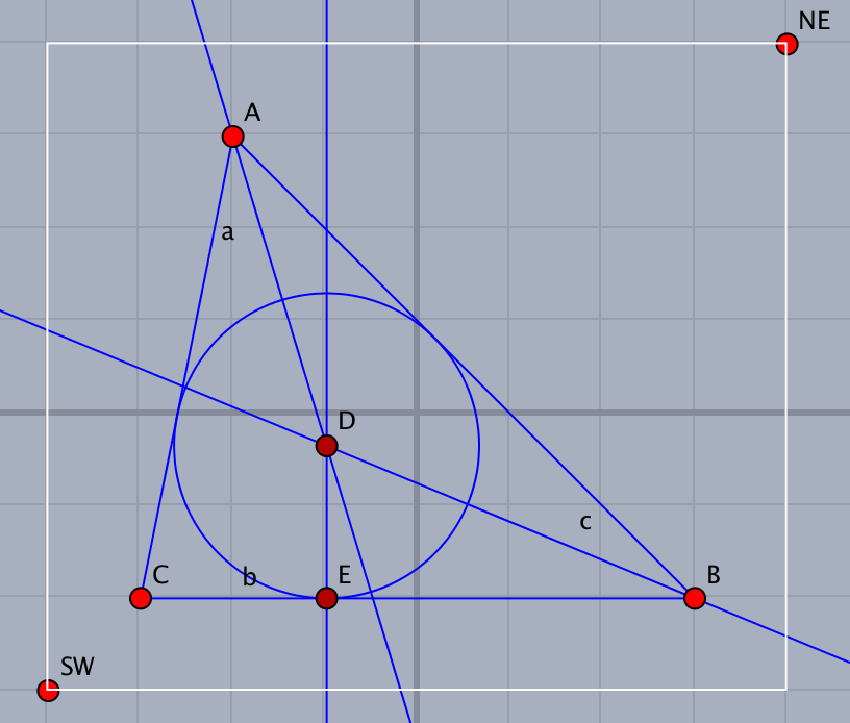
\includegraphics[bb=0.00 0.00 408.02 347.02,width=6cm]{Fig/incenter01.pdf}

\item 
Input the \ketcindy\ codes into Cindyscript editor 
to specify the graphical elements to be displayed 
in \TeX\ final output. 
Also \ketcindy\ codes are used 
to generate supplementary graphical elements 
and handle them. 

\hspace{10mm}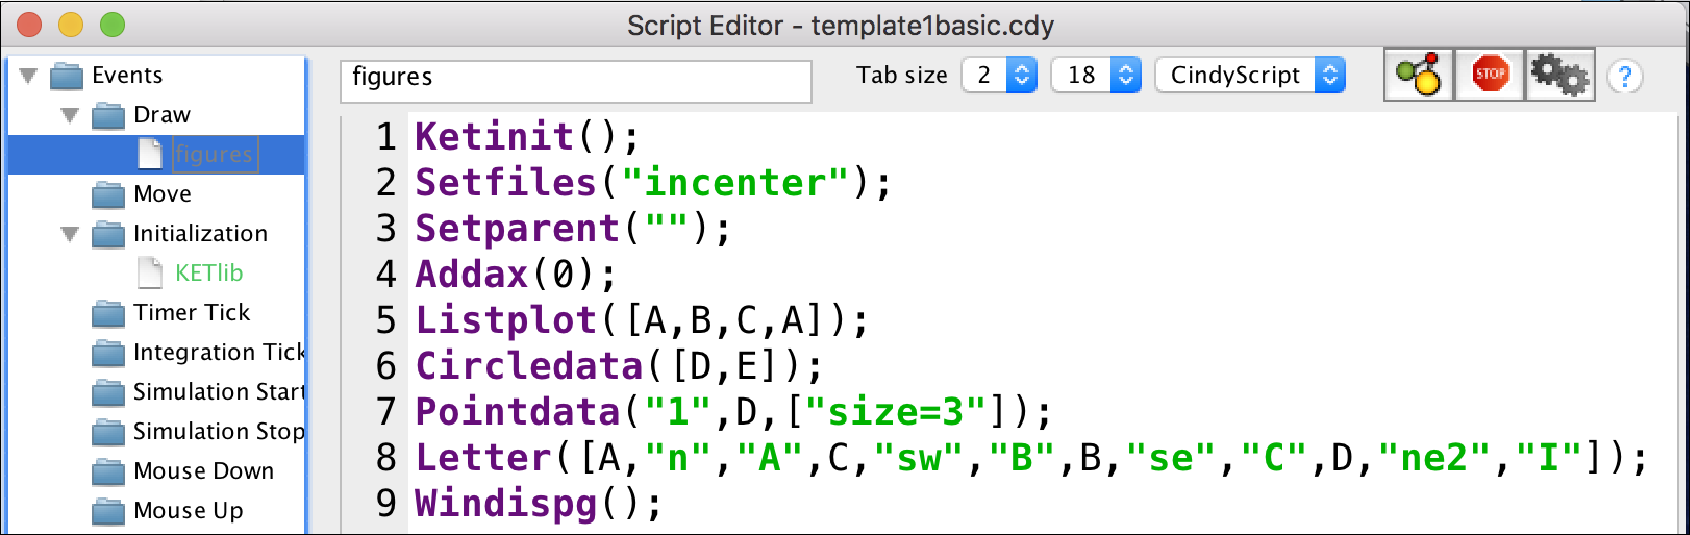
\includegraphics[bb=0.00 0.00 811.04 257.01,width=12cm]{Fig/incenter02E.pdf}

In this stage, the programming capabilities 
inherently implemented to Cindyscript can be used simultaneously. 
Execute the whole program by clicking the "Run" button. 
For more details, see section 3. 

\item 
Click the button named \verb|Figures| in Euclidean view 
to automatically generate the following files 
in the folder named "fig". 
Here, "incenter" is the name specified 
via the command \verb|Setfiles("incenter")| 
in step (2). 

\begin{tabbing}
12\=1234567897890123456\=\kill

 \> \verb|kc|.sh or \verb|kc.bat| \> shell script file(Mac) or batch file(Windows) \\
 \> \verb|incenter.r| \> \\
 \> \verb|incenter.tex| \> \TeX\ file composed of graphical codes\\
 \> \verb|incentermain.aux| \> \\
 \> \verb|incentermain.log| \> \\
 \> \verb|incentermain.pdf| \> PDF file to display the resulting graphical image\\
 \> \verb|incentermain.tex| \> \TeX\ file temporarily used to generate 
the file \verb|incentermain.pdf|
\end{tabbing}

Subsequently, the file \verb|incentermain.pdf| 
is automatically displayed as shown below. 

\hspace{30mm}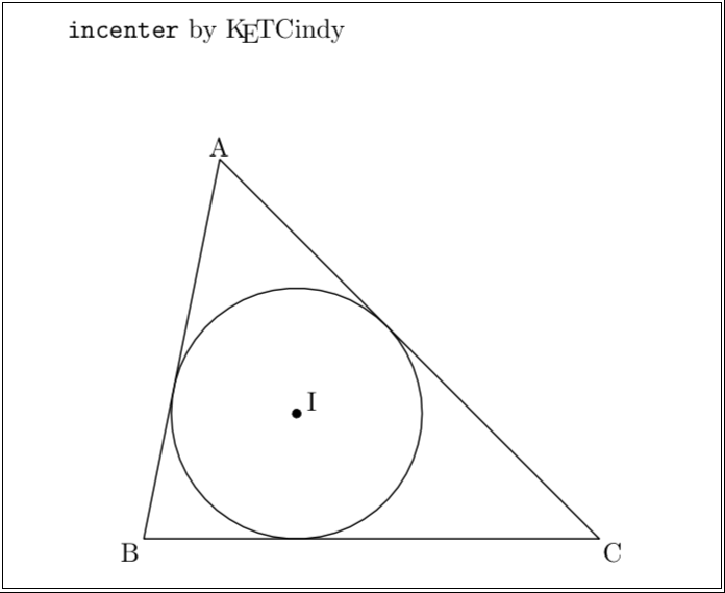
\includegraphics[bb=0.00 0.00 348.02 284.51,width=6cm]{Fig/incenter03.pdf}

We can manipulate this final output 
by modifying the inputs in steps (1) and (2) 
before processing the step (3) again. 

\vspace{\baselineskip}
\item  
Using \ketpic\ package of \TeX , 
\verb|incenter.tex| can be read 
into the targetting \TeX\ document 
via the command 
\begin{center}
\verb|\input{incenter}|
\end{center} 
Then the same figure is embedded in the targetting PDF output. 

\end{enumerate}


\newpage

\subsection{The drawing procedure of \ketcindy}

\subsubsection{Geometric figure}

\subsubsection{Graph of function}

\subsubsection{Spatial figure}

\subsubsection{Table}

\subsubsection{Collaboration with other software}


\newpage

\subsection{Plotting data}
Here we call the data computed 
to generate the graphs of functions and geometric elements 
"Plotting data" which is abbreviated as PD. 
The PD to draw segment is the list of coordinates 
of its two endpoints. 
For example, 
when the coordinates of the points A and B 
are (1, 1) and (3, 2) respectively, 
PD of the segment AB named \verb|Listplot ([A,B])| 
is stored in the form \verb|[[1,1],[3,2]]|. 
Also the PD to draw a curve is the collection of 
those for drawing small segments 
which connect contiguous dividing points of the curve. 
PD are automatically given names via \ketcindy\ 
following the rules below.

\begin{itemize}
\item 
The beginning part of the PD's name 
depends on the kind of the corresponding graphical element. 
For instance, 
\verb|sg| is associated to segments and 
\verb|cr| is associated to circles. 

\item 
When some extra name is specified 
as the first argument in the definition of PD, 
it is added to the beginning part given above. 
For instance, the PD defined below 
is given the name \verb|sg1|. 
\begin{center}
\verb|Listplot("1",[[0,0],[1,2]]);| 
\end{center}

\item 
When the extra name is not needed, 
the names of the points are added 
to the beginning part given above. 
For instance, the PD defined below  
is given the name \verb|sgABC|. 
\begin{center}
\verb|Listplot([A,B,C]);|
\end{center}

\end{itemize}

\noindent 
Once PD are generated, 
their names are displayed on the console view of Cinderella. 
For instance, when the PD named \verb|sgABCA| is generated, 
the corresponding message is displayed as shown below. 

\begin{center}
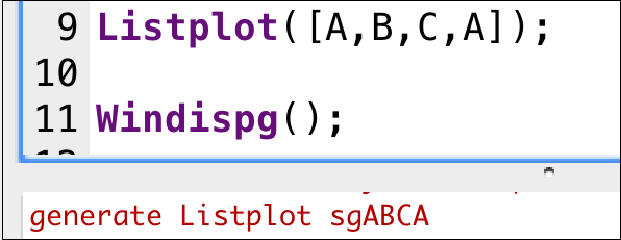
\includegraphics[bb=0.00 0.00 298.02 115.01,width=6cm]{Fig/pdtoconsole.pdf}
\end{center}
Also the content of PD is displayed 
via the function \verb|println()| of Cindyscript. 
For instance, inputting the command 
\verb|println(sgABCA)| makes the following list displayed. 
\begin{center}
\verb| [[1,3],[-1,0],[3,0],[1,3]] |
\end{center}
This list is composed of the coordinates of the points A, B, and C. 

These names of PD are used 
when the corresponding PD need to be transformed. 
For instance, 
PD to draw the parallel transport of the segment AB 
is generated via the \ketcindy\ command 
\begin{center}
\verb|Translatedata("1","sgAB",[2,3]);|
\end{center}

PD can be generated also 
by using the programming capability of Cindyscript 
which can be subsequently used in \ketcindy .  
For more details, 
see the example of \verb|Listplot()| 
in the command reference. 
Inclusion of too much elements into a single PD 
may cause some error. 
To prevent such error, 
PD should be divided into several PD 
each of which is composed of 200 elements or so. 


\newpage

\section{Cindyscript}

\subsection{Cindyscript editor}

Choose "Cindyscript" in the "Scripting" menu 
or push keybuttons Ctrl+9 (Windows) / Command+9 (Mac), 
then Cindyscript editor opens as shown below. 

\begin{layer}{150}{0}
\putnotese{7}{15}{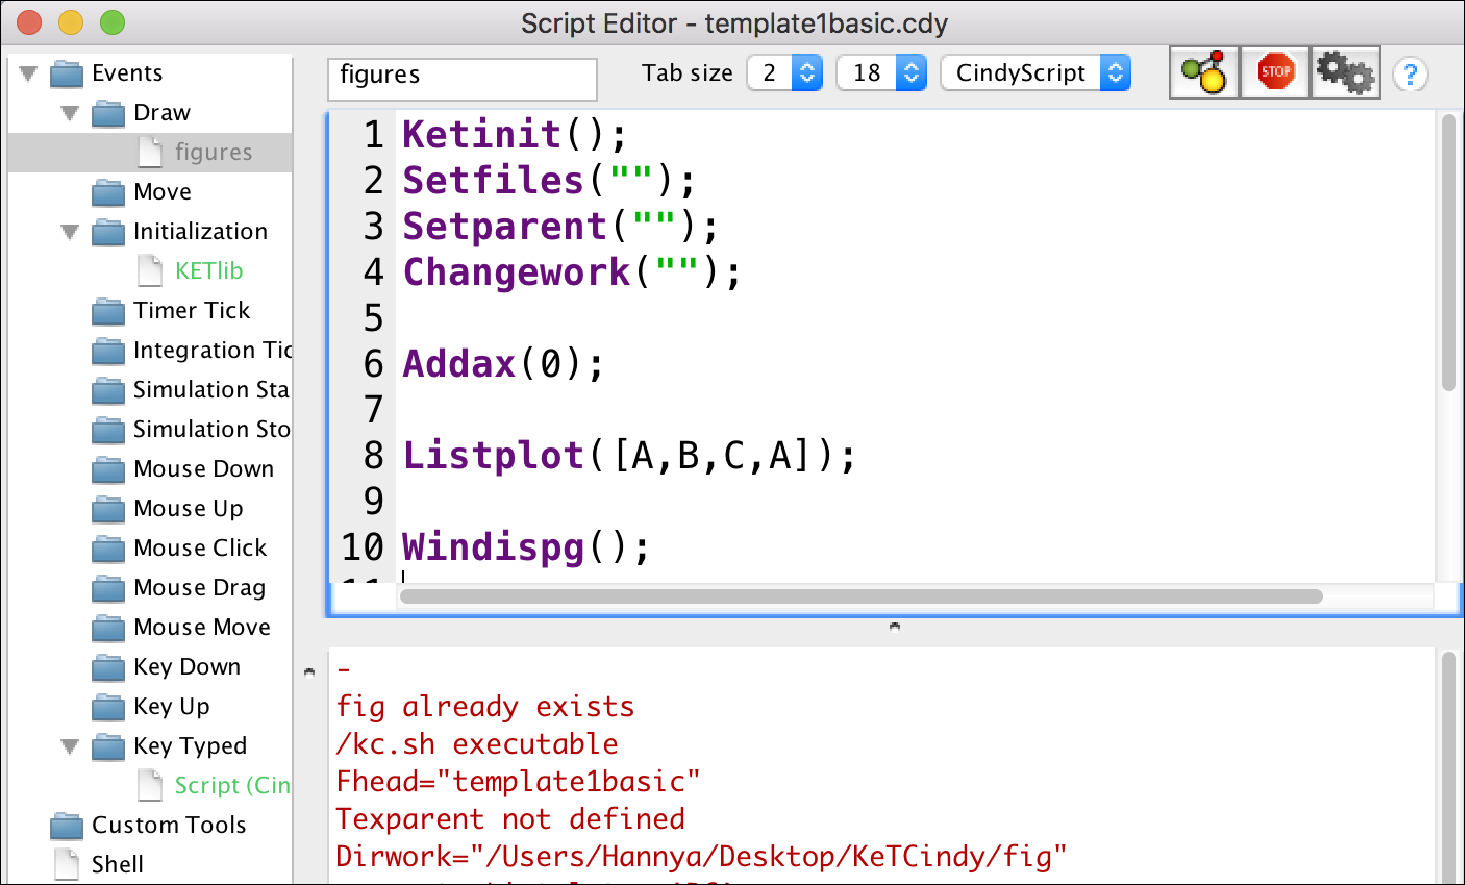
\includegraphics[bb=0.00 0.00 703.04 425.02,width=14cm]{Fig/slotE.pdf}}
\arrowlineseg[16]{30}{20}{10}{90}
\putnotese{25}{5}{Slots}
\arrowlineseg[16]{50}{20}{10}{100}
\putnotese{42}{5}{Page name}
\arrowlineseg[16]{90}{20}{10}{110}
\putnotese{80}{5}{Font size}
%\arrowlineseg[16]{107}{20}{15}{140}
%\putnotese{80}{5}{描画面を前面に}
\arrowlineseg[16]{135}{20}{10}{110}
\putnotese{125}{5}{Run}
\arrowlineseg[16]{142}{20}{10}{100}
\putnotese{135}{5}{Help}
\putnotese{100}{35}{Text field}
\putnotese{100}{80}{Console}
\end{layer}

\vspace{105mm}

Commands can be input into preferred "slot". 
Specific timing for execution of commands 
is assigned to each slot. 
The slot for current work can be chosen 
only by clicking the corresponding tab in the menu. 
Users can add extra pages to each slot. 
For instance, 
when some initialization other than 
those included in \verb|KETlib| is needed, 
clicking the folder icon of "Initialization" makes a new page open 
in which extra commands can be input. 
The name of each page can be given 
by directly inputting it into the "Page name" column. 
The font size of the scripts can be tuned 
by changing the number in the "Font size" column. 
Frequently used slots are listed below. 

\begin{itemize}

\item 
Draw

The commnds in this slot are executed 
when some change, like movement of point, 
occurs in the Euclidean view. 
In \verb|templatebasic1.cdy|, 
the protoype page named \verb|figure| 
including the \ketcindy\ commnads 
like \verb|Ketinit();| and \verb|Windispg();| 
which are unconditionally necessary 
has been prepared.  
The \ketcindy\ commands for drawing 
should be input into this slot. 

\item 
Initialization 

The definitions of functions 
and the initial values of variables 
are input here. 
The commands in this slot are exected 
only once just after the "Run" button is clicked. 
Thus, the initial data in this slot is changed 
when some modifications are made in other slots. 
In \verb|templatebasic1.cdy|, 
the protoype page named \verb|KETlib| 
including the default setting of \ketcindy\ 
has been prepared. 

\item 
Key Typed

The commnds in this slot are executed 
when some key is pushed. 

\end{itemize}

Clicking "Run" button or pushing the keybuttons Shift+Enter 
makes the whole program be executed. 
The results derived from executing the function \verb|print()| 
and error messages are displayed on the console view 
which is put at the bottom part of Cindyscript editor. 
Each error and its location 
is displayed together with the message 
"WARNING" or "syntax error". 
The outputs displayed on the console 
can be copied to other usual text editors. 

Click the "Help" button, 
then reference manual of Cinderella opens 
as shown below. \\

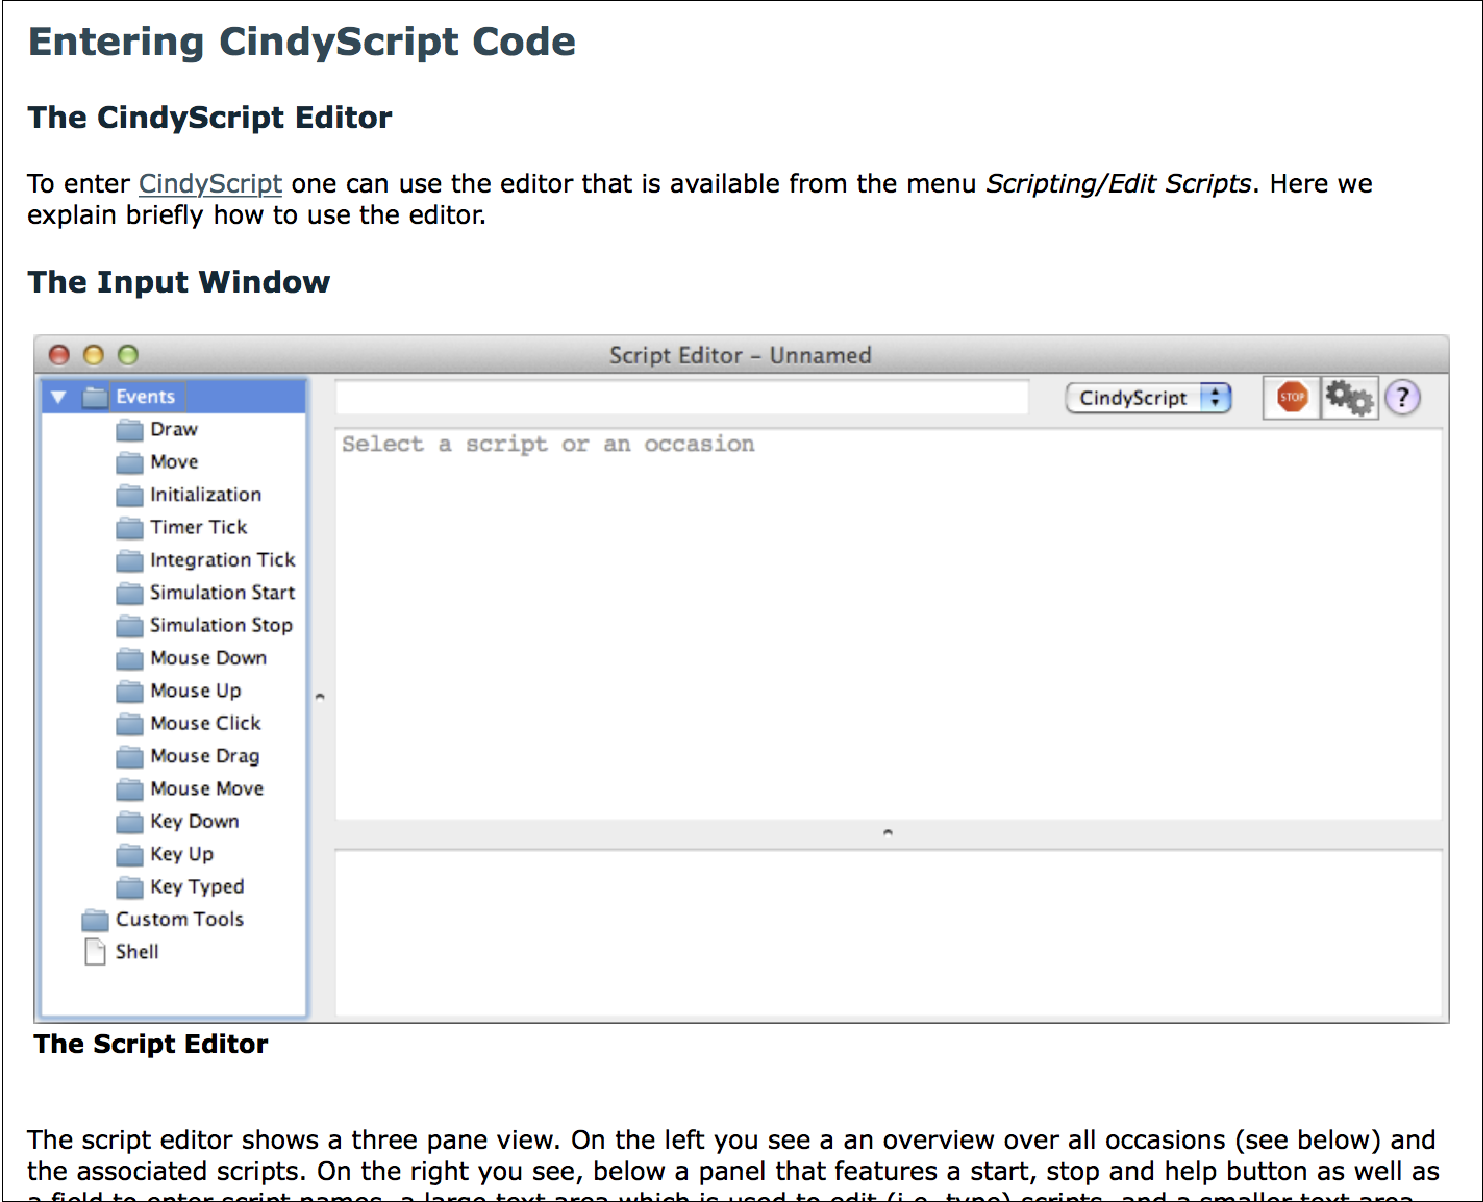
\includegraphics[bb=0.00 0.00 712.04 577.03,width=14cm]{Fig/CindyhelpE.pdf}




\subsection{Input}


\subsection{Variables and constants}


\subsection{Frequently used commands}





% -------------- Making slide --------------

\newpage

\section{Making Slides}

\subsection{Overall Flow}

\ketcindy\ has functions to make slides for presentation. 
For this, follow steps below:
\begin{enumerate}[1)]
\item Copy and rename \verb|template2slide.cdy| in ketcindy folder to a work folder and double-click the file (here, we call sample.cdy). Then the followings will appear.
\begin{center}
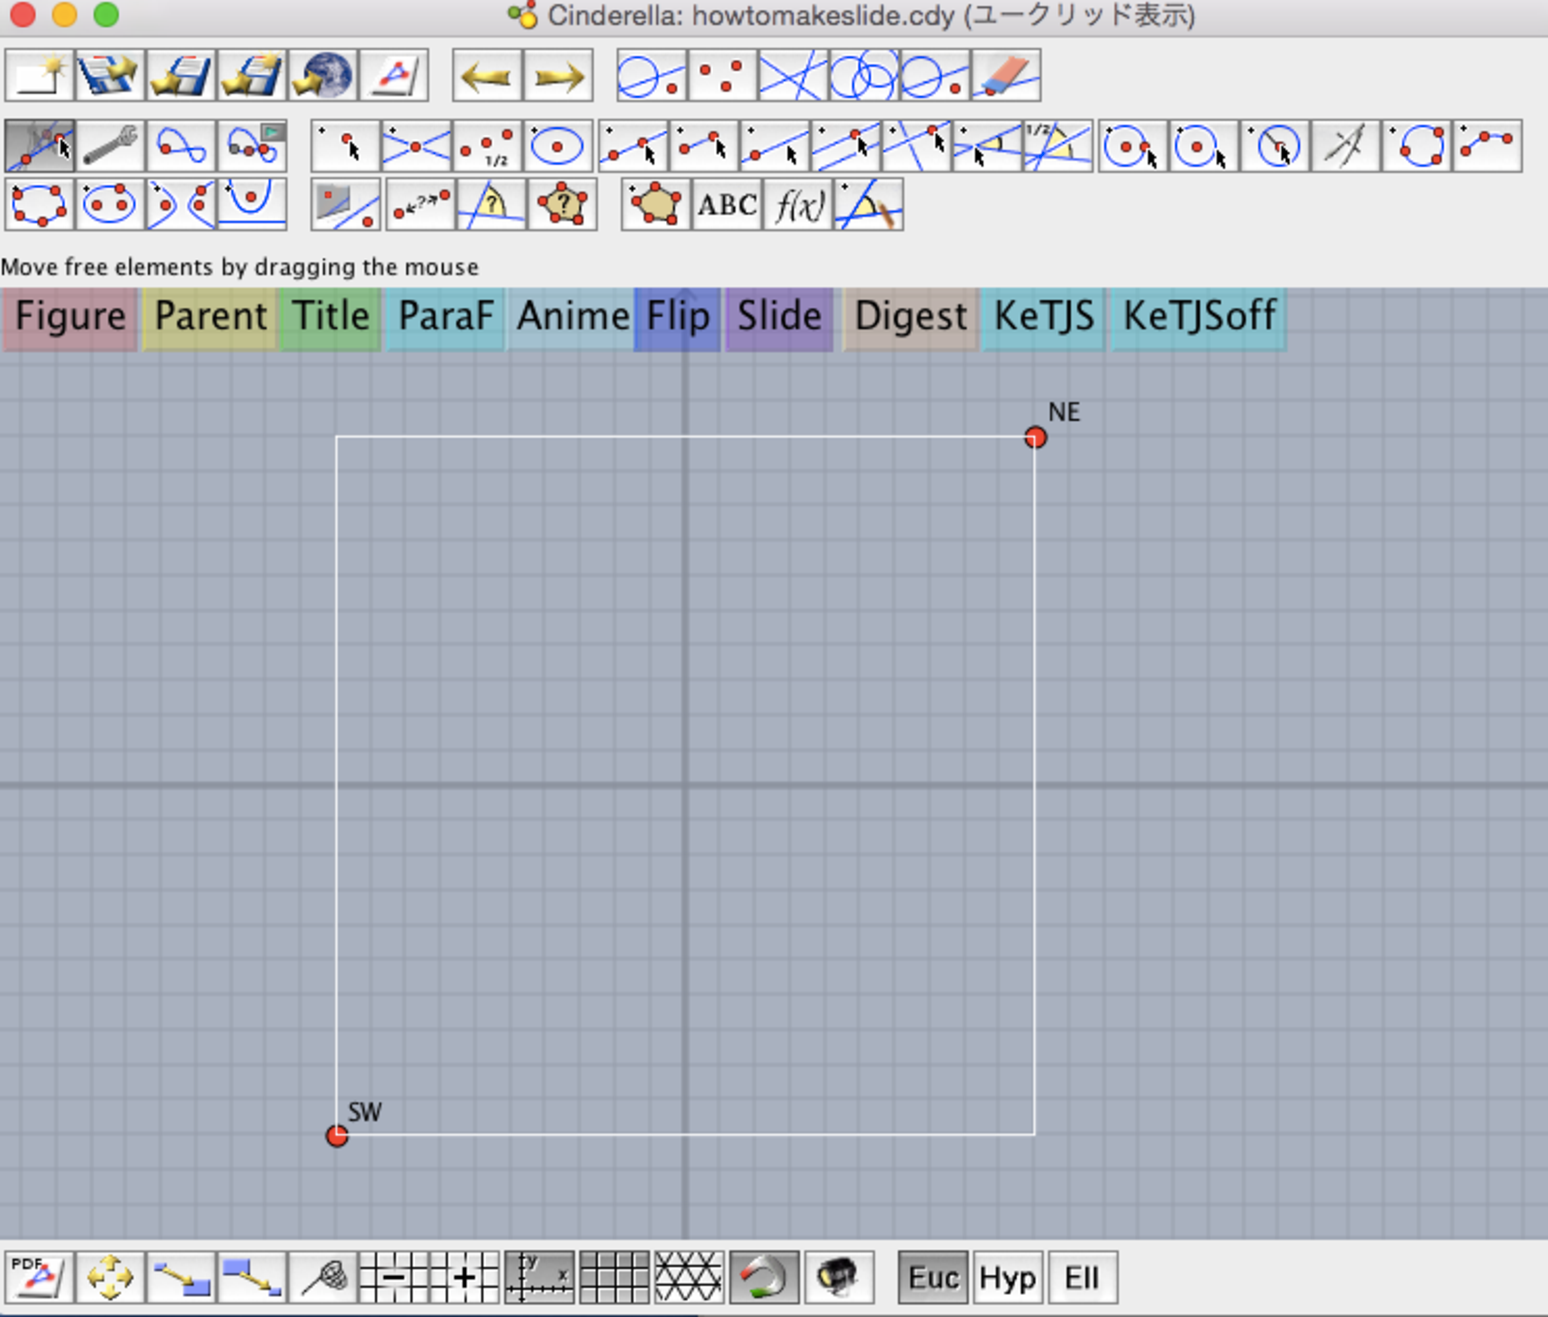
\includegraphics[bb=0.00 0.00 743.00 632.00,height=60mm]{fig/slidescreen.pdf}\hspace{5mm}
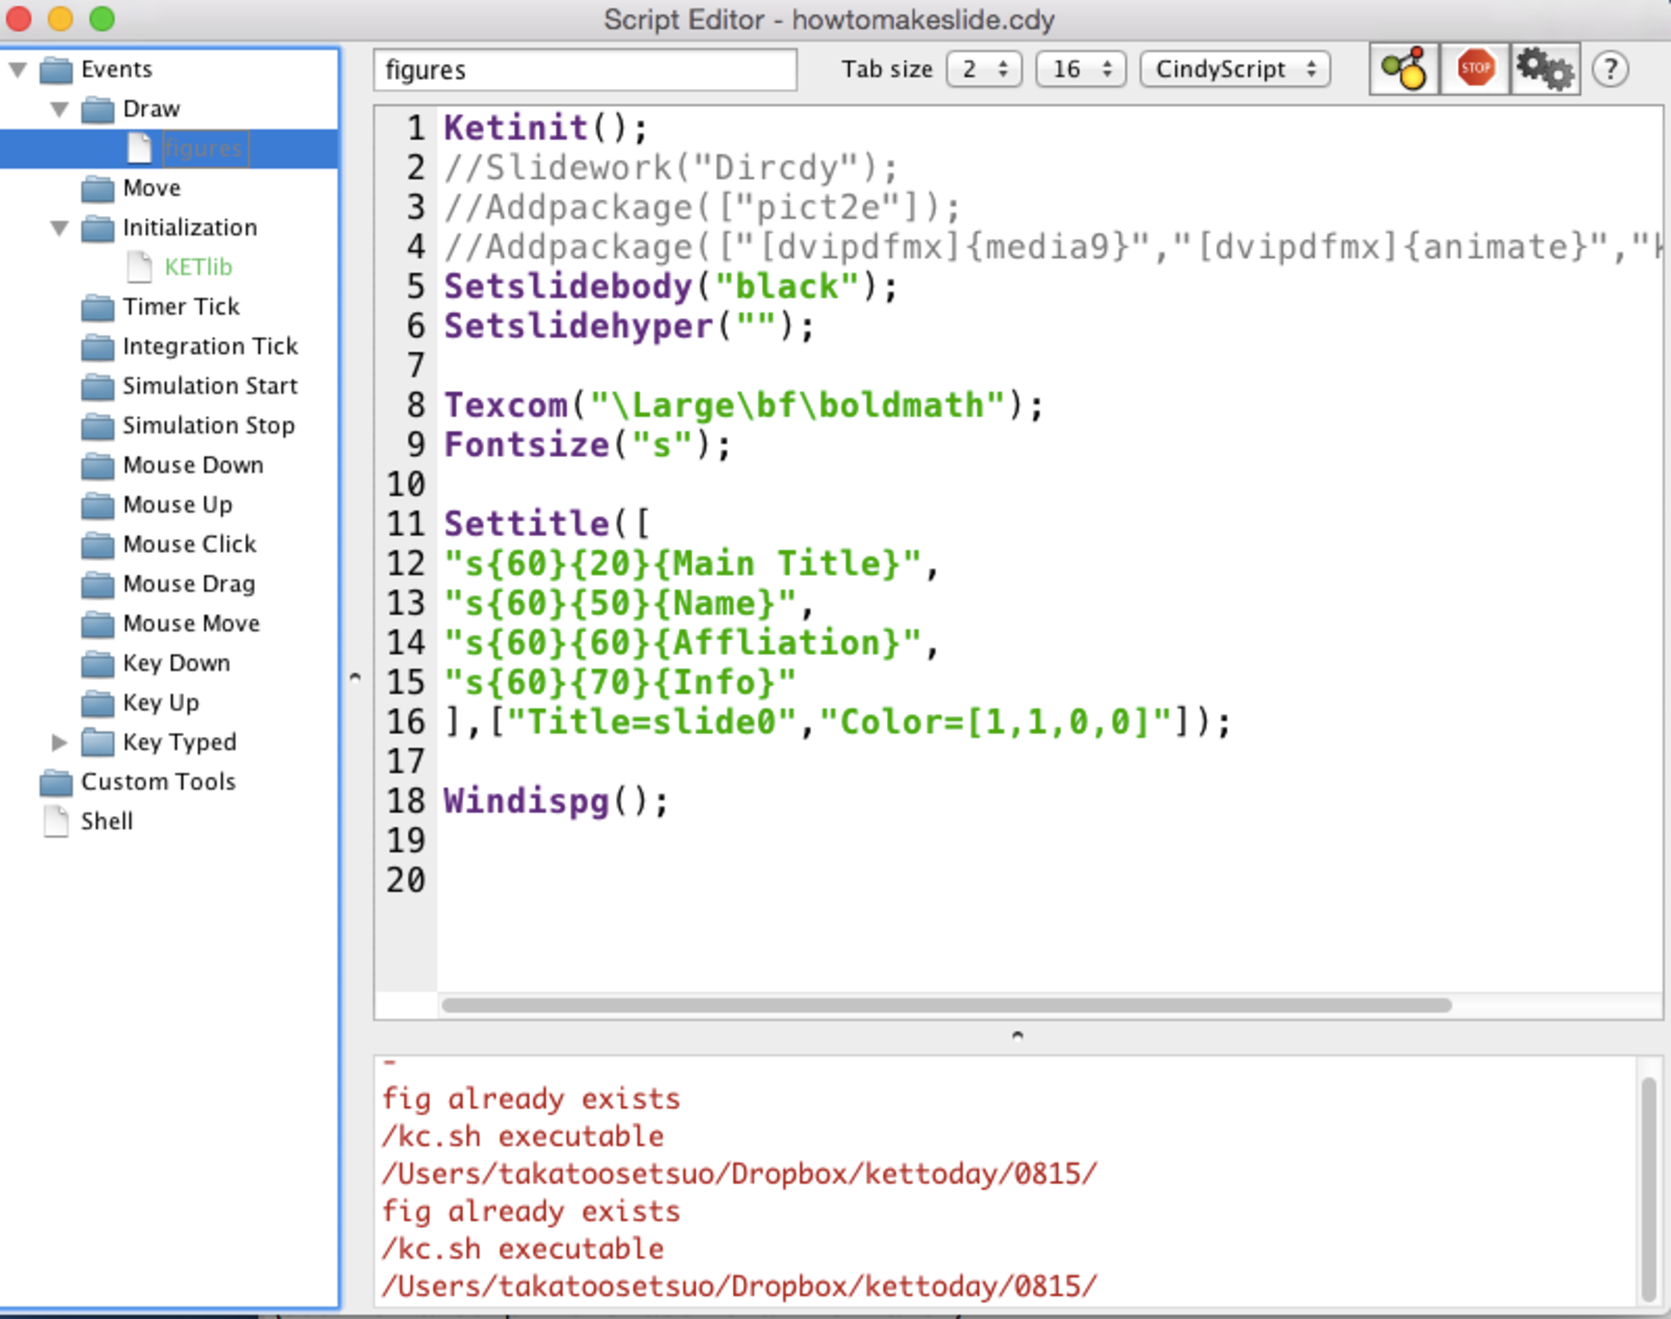
\includegraphics[bb=0.00 0.00 802.00 633.00,height=60mm]{fig/slidescript.pdf}
\end{center}
\item Edit \verb|"Settitle"|, for example,\\
\verb|  Settitle([|\\
\verb|     "s{60}{20}{How To Use}",|\\
\verb|     "s{60}{50}{a \ketcindy\ member}",|\\
\verb|     "s{60}{60}{\ketcindy\ project}",|\\
\verb|     "s{60}{70}{Aug. 20th}"|\\
\verb|    ],["Color=[1,1,0,0]"]);|
\item Press button \verb|"Title"|, then the title page will be displayed. At the same time,  text file \verb|"sample.txt"| will be created if it does not exist. This \verb|sample.txt| is a template file for making slides.
\item Press button \verb|"Slide"|, then \ketcindy\ will make \verb|sample.tex| from \verb|sample.txt|, 
typeset it, and display \verb|sample.pdf| which contains slides for presentation.
\end{enumerate}
 
\subsection{Editing Text File}

\begin{enumerate}[1)]
\item Put \verb|//| at the last of each line.\\
\hspace*{10mm}Rm) Use \verb+||||+ for \verb|//|.
\item Commands are\\
\verb|    title::titleslidename(::wallpaper)//|\\
\verb|        Rem) Put only once at the first line.|\\
\verb|    main::(main title)//|\\
\verb|    new::(page title)//|\\
\verb|    enumerate//|\\
\verb|           =\begin{enumerate}|\\
\verb|        Rem) Add the option such as [(1)] using :: .|\\
\verb|    itemize//|\\
\verb|           =\begin{itemize}|\\
\verb|    layer::{xsize}{ysize}//|\\
\verb|           =\begin{layer}{xsize}{ysize}|\\
\verb|         Rem) "layer" is an environment defined in ketlayer.sty.|\\
\verb|    item::sentence//|\\
\verb|           =\item sentence|\\
\verb|    putnote::dir{xpos}{ypos}::filename(,scale)//|\\
\verb|           =putnotedir{xpos}{ypos}{\input{fig/filename}}||\\
\verb|         Rem) "putnote" is a command defined in ketlayer.sty|\\
\verb|    end//|\\
\verb|           =\end{itemize,enumerate,layer}|\\
\verb|    ...//|\\
\verb|          To insert a blank line.|\\
\verb|    Rem) Any other TeX command is available.|\\
\end{enumerate}

\subsection{Display of Page step by step}

\begin{enumerate}[1)]
\item Put just after new,\\
\verb|    %repeat=number of steps//|
\item Put at the head of each line as\\
\verb|    %[2,-]::sentence|\\
\verb|          display at all steps from 2|\\
\verb|    %[-,2]::sentence|\\
\verb|           display at all steps until 2|\\
\verb|    %[1..3,5]::sentence|\\
\verb|           display at steps of 1,2,3 and 5|
\item  Use \verb|%thin| to display with thin letters.\\
\verb|    %thin::[2,-]::sentence|
\item The dencity can be changed with Setslidebody or \verb|\setthin|.
\end{enumerate}

\subsection{Making Flip Animation}

\begin{enumerate}[1)]
\item Define function \verb|Mf(s)|, the state at s.
\item Put command \verb|Setpara| in the script editor as\\ 
\verb|    Setpara(subfolder,funcitonstr(mf(s)),range,options);|\\
\verb|        options=["m/r", "Div=25"];|
\item Describe in the text file as\\
\verb|    %repeat=, para=subfolder:{0}:s{60}{10}:input(:scale)//|
\item Press buttons \verb|ParaF| and \verb|Flip|, then \verb|subfolder| will be generated.
\item Press button \verb|Slide|.
\end{enumerate}

\subsection{Making Animation}

\begin{enumerate}[1)]
\item Add the following in the script editor\\ 
\verb|    Addpackage(["[dvipdfmx]{animate}"]);|
\item Add in the second option of Setpara,\\
\verb|    "Frate=num of frame in the second,"Scale=scale,"OpA=option of animation" |
\item Press buttons \verb|ParaF| and \verb|Anime|, then \verb|subfolder| will be generated.
\item Use \verb|\input|, not layer, to display.
\end{enumerate}

\subsection{Changing Style}

The default styles such as size and color of letters can be changed.
See \verb|KeTCindyReferenceE|.

\end{document}